%\graphicspath{{/Users/emiliendurif/Documents/prepa/sujets/DS/flir/images/}}
%\vspace{-1.5cm}
\begin{huge}
\textbf{Vision en réalité augmentée pour hélicoptère}
\end{huge}

\subsection{Présentation du système}

\subsubsection{Contexte}
\begin{figure}[h]
\begin{center}
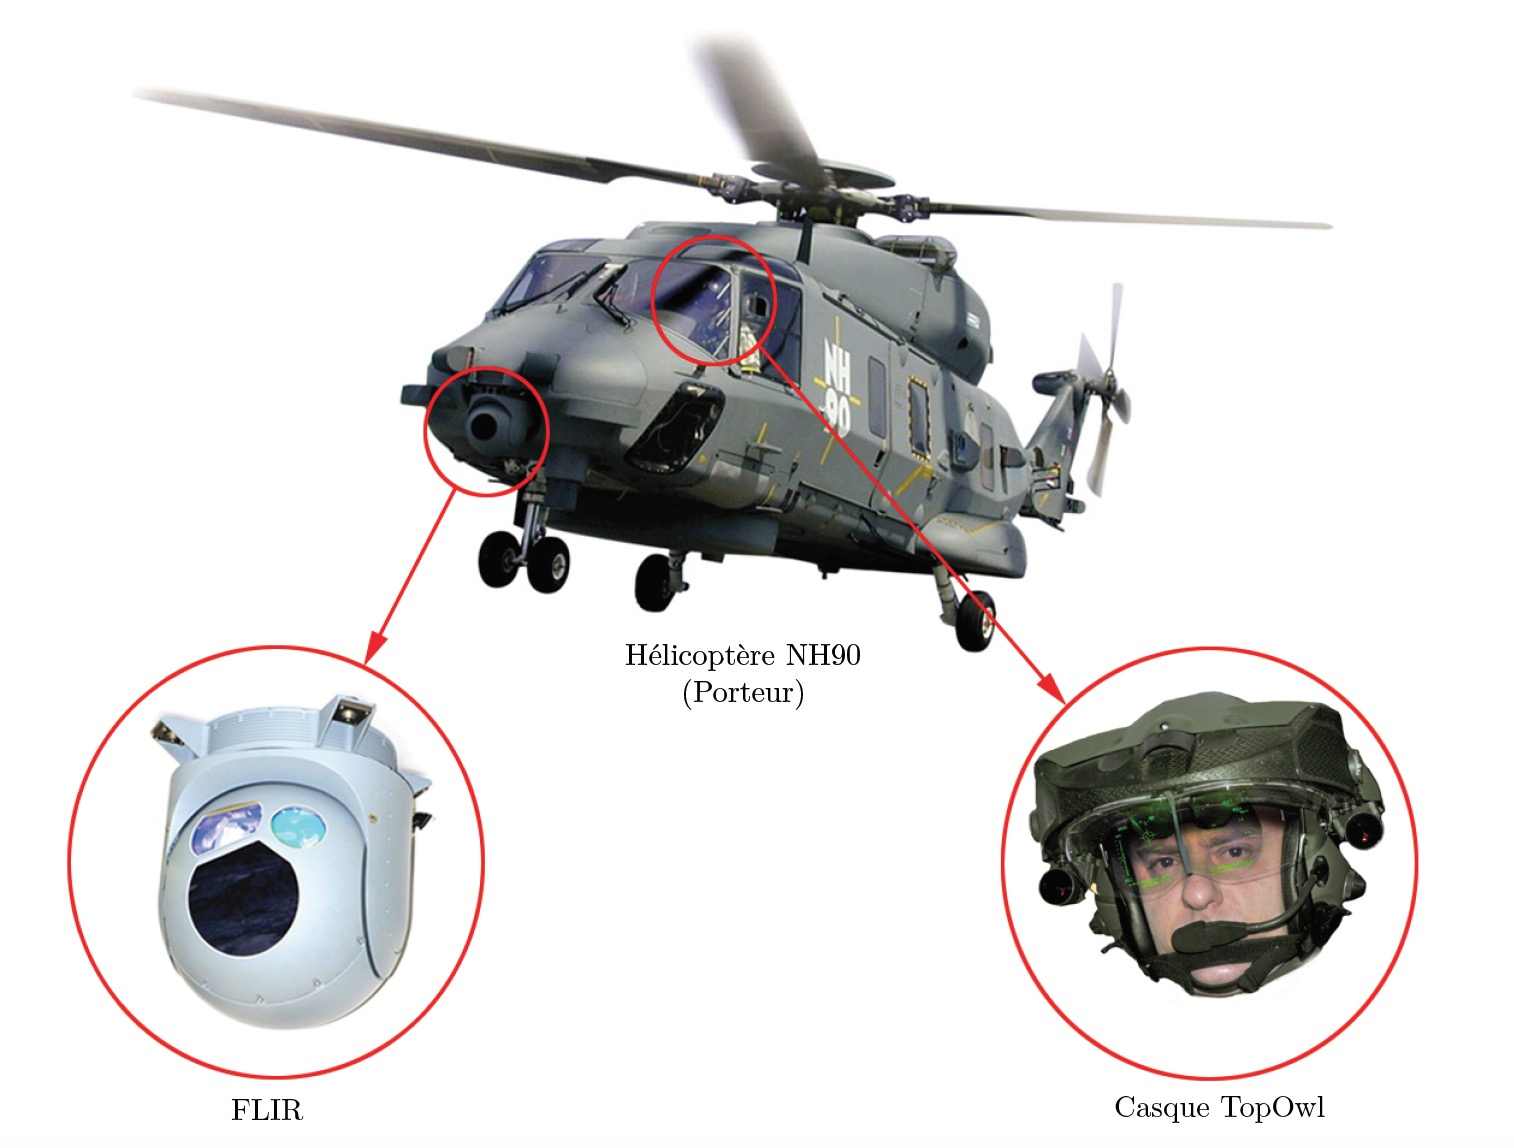
\includegraphics[width=0.6\textwidth]{figure1.jpg}
\caption{Hélicoptère NH90 équipé du système de vision en réalité augmentée\label{fig1}}
\end{center}
\end{figure}

\begin{figure}[!htb]
\begin{center}
\begin{minipage}{0.45\textwidth}
Les hélicoptères sont des aéronefs dont l'un des intérêts
est de pouvoir effectuer des vols proches du relief. Suivant
les conditions climatiques (tempête de sable, brouillard
ou vol de nuit par exemple), la propre vision du pilote
et l'instrumentation de navigation classique peuvent être
insuffisantes pour assurer la sécurité du vol. Pour pallier
cela, la société Thalès propose un système de vision en
réalité augmentée composée du casque TopOwl et d'un
FLIR (\textit{Forward Looking InfraRed}).
\end{minipage}
\begin{minipage}{0.45\textwidth}
\begin{center}
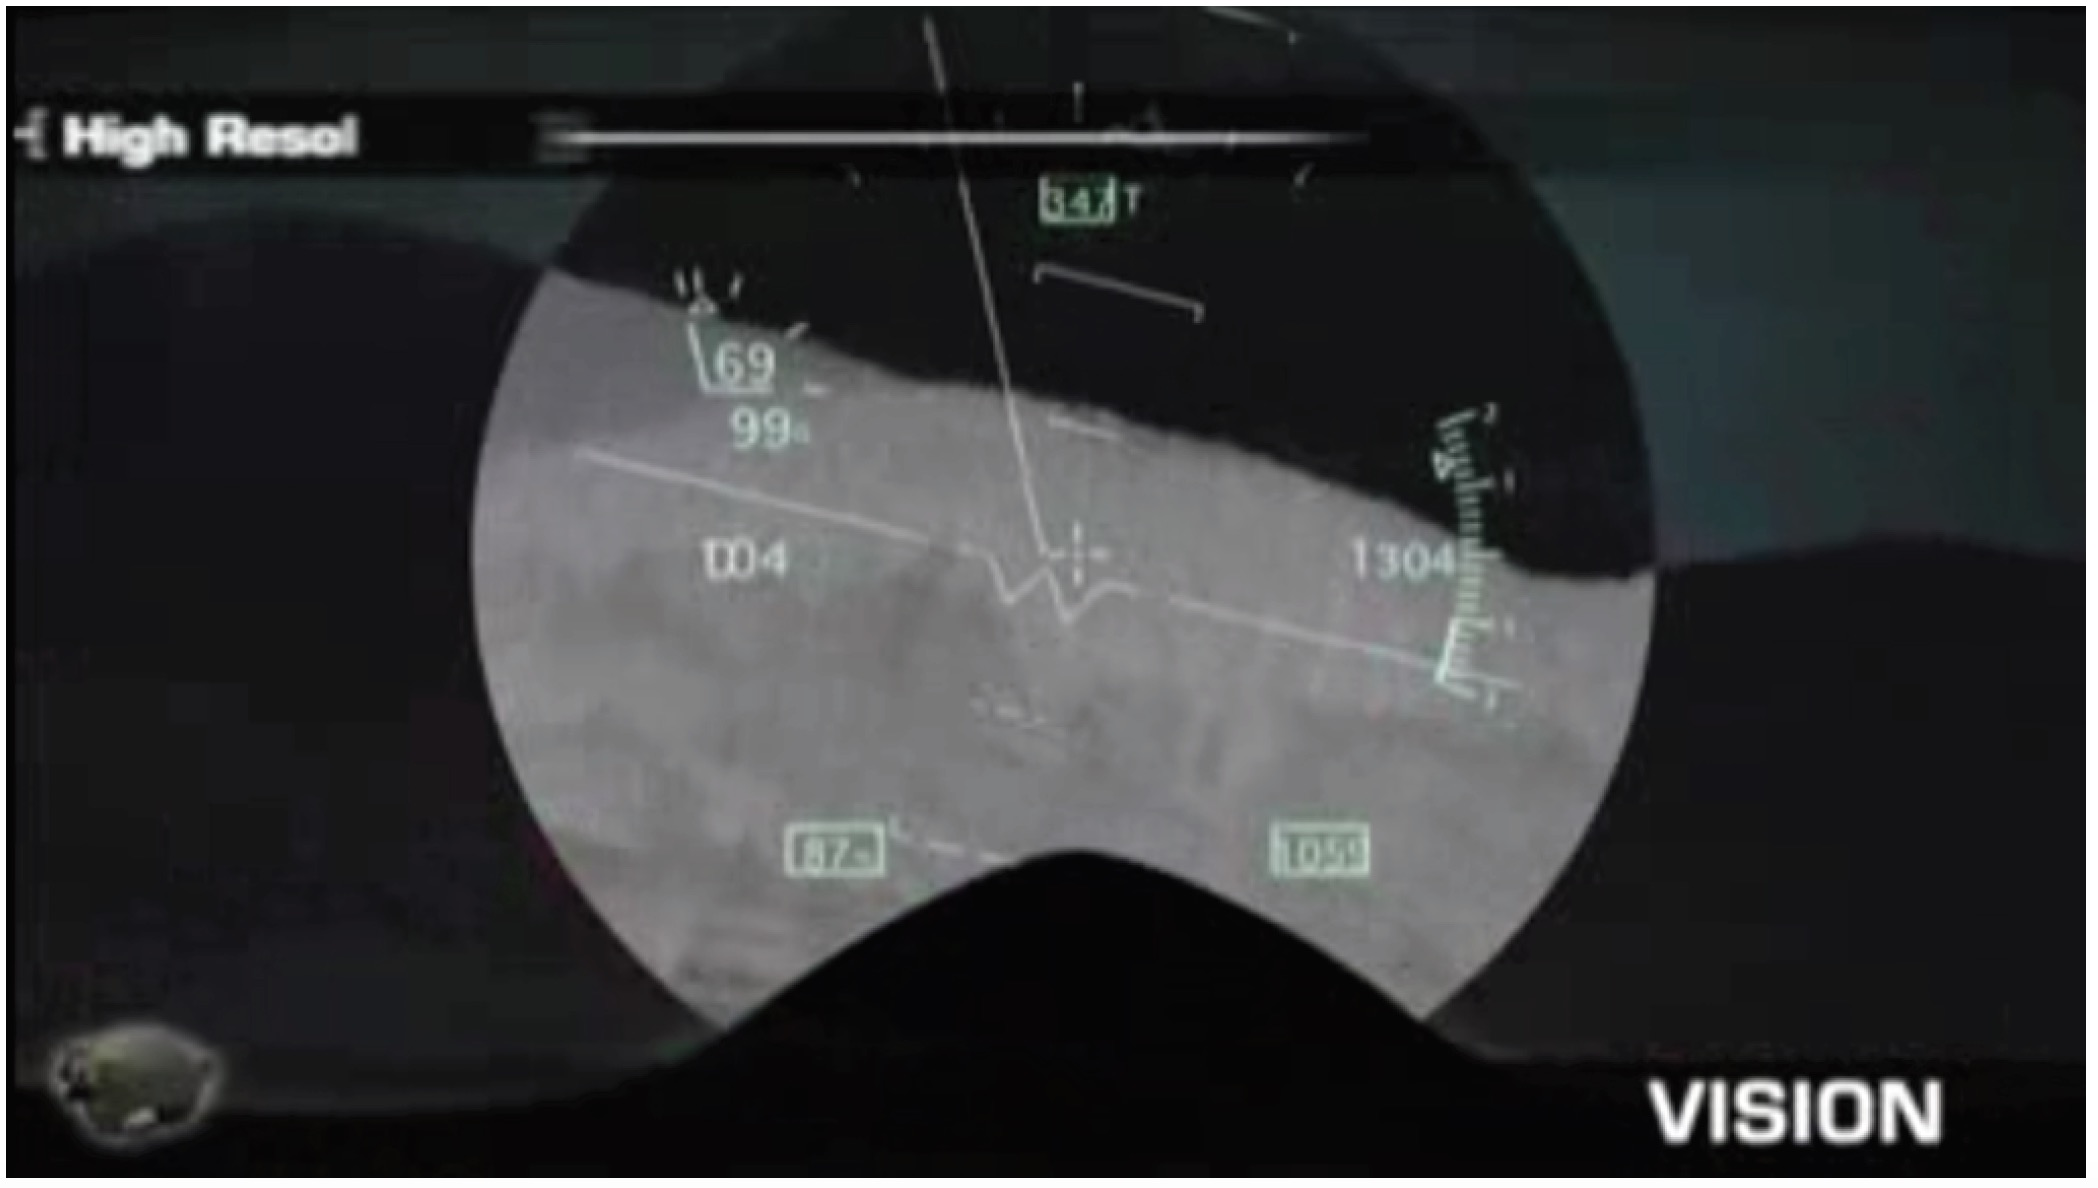
\includegraphics[width=0.8\textwidth]{figure2.jpg}
\caption{Hélicoptère NH90 équipé du système de vision en réalité augmentée\label{fig2}}
\end{center}
\end{minipage}
\end{center}
\end{figure}

%\FloatBarrier
La vision en réalité augmentée consiste à venir projeter
sur la visière du casque TopOwl une image prise par une
des caméras du \textbf{FLIR}. L'image projetée se superpose au
paysage visible à travers la visière de façon à améliorer
la vision du pilote. De nuit, par temps de brouillard ou
de tempête, l'image peut être une image infra-rouge ou
thermique. En plus de l'image, des informations peuvent être ajoutées sur la projection ; par exemple des données
GPS, des routes, des informations de vol.

Le FLIR est une boule optronique modulaire pouvant intégrer plusieurs capteurs différents dont une caméra
thermique, une caméra couleur TV HD, ainsi qu'une caméra très bas niveau de lumière. Cet ensemble est
orientable et gyrostabilisé, c'est-à-dire en particulier que les caméras sont capables de garder une même ligne
de visée par rapport au référentiel terrestre, quels que soient les mouvements de l'hélicoptère NH90 qui sera
appelé \textbf{porteur} dans la suite du sujet. Le casque TopOwl est placé sur la tête du pilote et le \textbf{FLIR} sur l'avant
du porteur.
Une étude relative à la physique du casque TopOwl a permis de déterminer certaines de ses performances qui
seront données au moment opportun. Ce sujet a pour objet l'étude des performances du sous-système FLIR,
intégré dans le système de vision en réalité augmentée. La problématique globale est de vérifier que l'image
projetée sur la visière du casque TopOwl est utilisable par le pilote, c'est-à-dire :
\begin{itemize}
\item  que la ligne de visée des caméras est conforme à la ligne de visée du pilote (les lignes de visée sont définies
par rapport au référentiel terrestre) ;
\item que le retard entre la prise de vue et son affichage n'est pas visible par le pilote (retard inférieur à la
persistance rétinienne) ;
\item que la prise de vue n'est pas perturbée par les mouvements du porteur.
\end{itemize}


\subsubsection{Exigences}

\begin{figure}[!htb]
\begin{center}
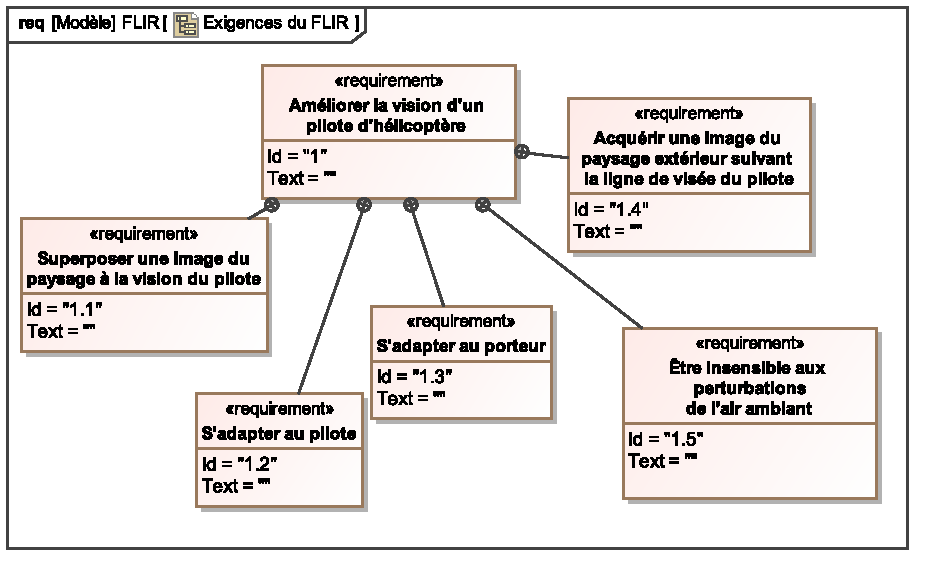
\includegraphics[width=0.7\textwidth]{req_flir.pdf}
\caption{Diagramme des exigences partiel \label{req_flir}}
\end{center}
\end{figure}


\begin{table}[!htb]
\begin{center}
\begin{tabular}{|p{0.3\textwidth}|p{0.3\textwidth}|p{0.3\textwidth}|}
\hline 
\textbf{Exigence} & \textbf{Critère} & \textbf{Valeur} \\ 
\hline 
1.1 Superposer une image du paysage à la vision du pilote & Résolution (largeur du plus petit
objet visible sur l'image) & 1 m pour un objet situé à 1 km de
distance du pilote \\ 
\cline{2-3} 
& Précision (décalage entre l'image
projetée sur la visière du TopOwl et
le paysage réel) & Erreur de superposition inférieure
ou égale à 1 pixel\\ 
\cline{2-3}  
 & Latence d'affichage (temps entre la
prise de vue et son affichage sur la
visière du TopOwl) & Inférieure ou égale à la persistance
rétinienne ($t_{ret} \leq 120 ms$) \\ 
\cline{2-3}  
 & Stabilité de l'image projetée sur la
visière & Oscillations d'amplitude inférieure
à 1/2 pixel \\ 
\hline
\end{tabular} 
\caption{Cahier des charges partiel du système de vision en réalité augmentée \label{tab1}}
\end{center}
\end{table}

L'étude se décompose en trois parties. Une étude de la physique du casque TopOwl ayant été effectuée dans
le sujet de physique, la partie 2 porte sur la détermination des performances (rapidité et précision) à atteindre
par le sous-système FLIR en fonction du cahier des charges du système de vision en réalité augmentée et
des performances des autres sous-systèmes. L'objectif des parties 3 et 4 est d'analyser le choix d'architecture du
FLIR en vue de valider les hypothèses simplificatrices concernant son comportement. La partie 5 consiste à
vérifier si les solutions retenues, tant au niveau de l'architecture que de la commande, permettent d'atteindre
les performances attendues du FLIR

\subsection{Performances attendues du sous-système FLIR intégré au système
de vision en réalité augmentée}\label{partie1}

\begin{obj}
Déterminer les performances de rapidité et de précision d'orientation de la ligne de visée du sous-système
FLIR qui permettent de satisfaire le cahier des charges du système de vision en réalité augmentée
pour hélicoptère.
\end{obj}

\subsubsection{Validation des performances simulées du FLIR}

Le sous-système de détection de posture, appelé \textit{DDP}, placé sur le casque TopOwl permet d'acquérir l'orientation
spatiale de la tête du pilote par rapport au cockpit du porteur (3 angles de rotation). Cette information, couplée
à l'information de position et d'orientation du porteur par rapport à la Terre (délivrée par une centrale inertielle fixée au porteur), permet d'élaborer la commande d'orientation du FLIR afin que sa ligne de visée corresponde
à la ligne de visée du pilote. À partir d'un algorithme, une centrale de traitement d'image permet de calculer
l'image à afficher sur la visière du casque TopOwl et les informations éventuelles à ajouter, comme celles issues
de la position GPS par exemple.

\subsubsection{Détermination des performances du FLIR}

Le système de détection de posture (DDP) a besoin d'un temps noté $t_{ddp}$ égal à $20 ms$ pour acquérir l'information. De même, le temps de traitement de l'information par filtrage noté $t_{filtre}$ est égal à $5 ms$.
On donne les temps suivants pour la réalisation des tâches :
\begin{itemize}
\item les temps d'acquisition des informations par les capteurs autres que la DDP sont négligeables devant les
autres temps ;
\item le temps d'acquisition de l'image par les caméras du FLIR est négligeable devant les autres temps ;
\item le temps de traitement des informations issues des caméras du FLIR (traitement des images) est noté
$t_{trait}$ = 50 ms maximum ;
\item le temps mis par le TopOwl pour afficher l'image est noté $t_{com} = 5 ms$.
\end{itemize}

\begin{figure}[!htb]
\begin{center}
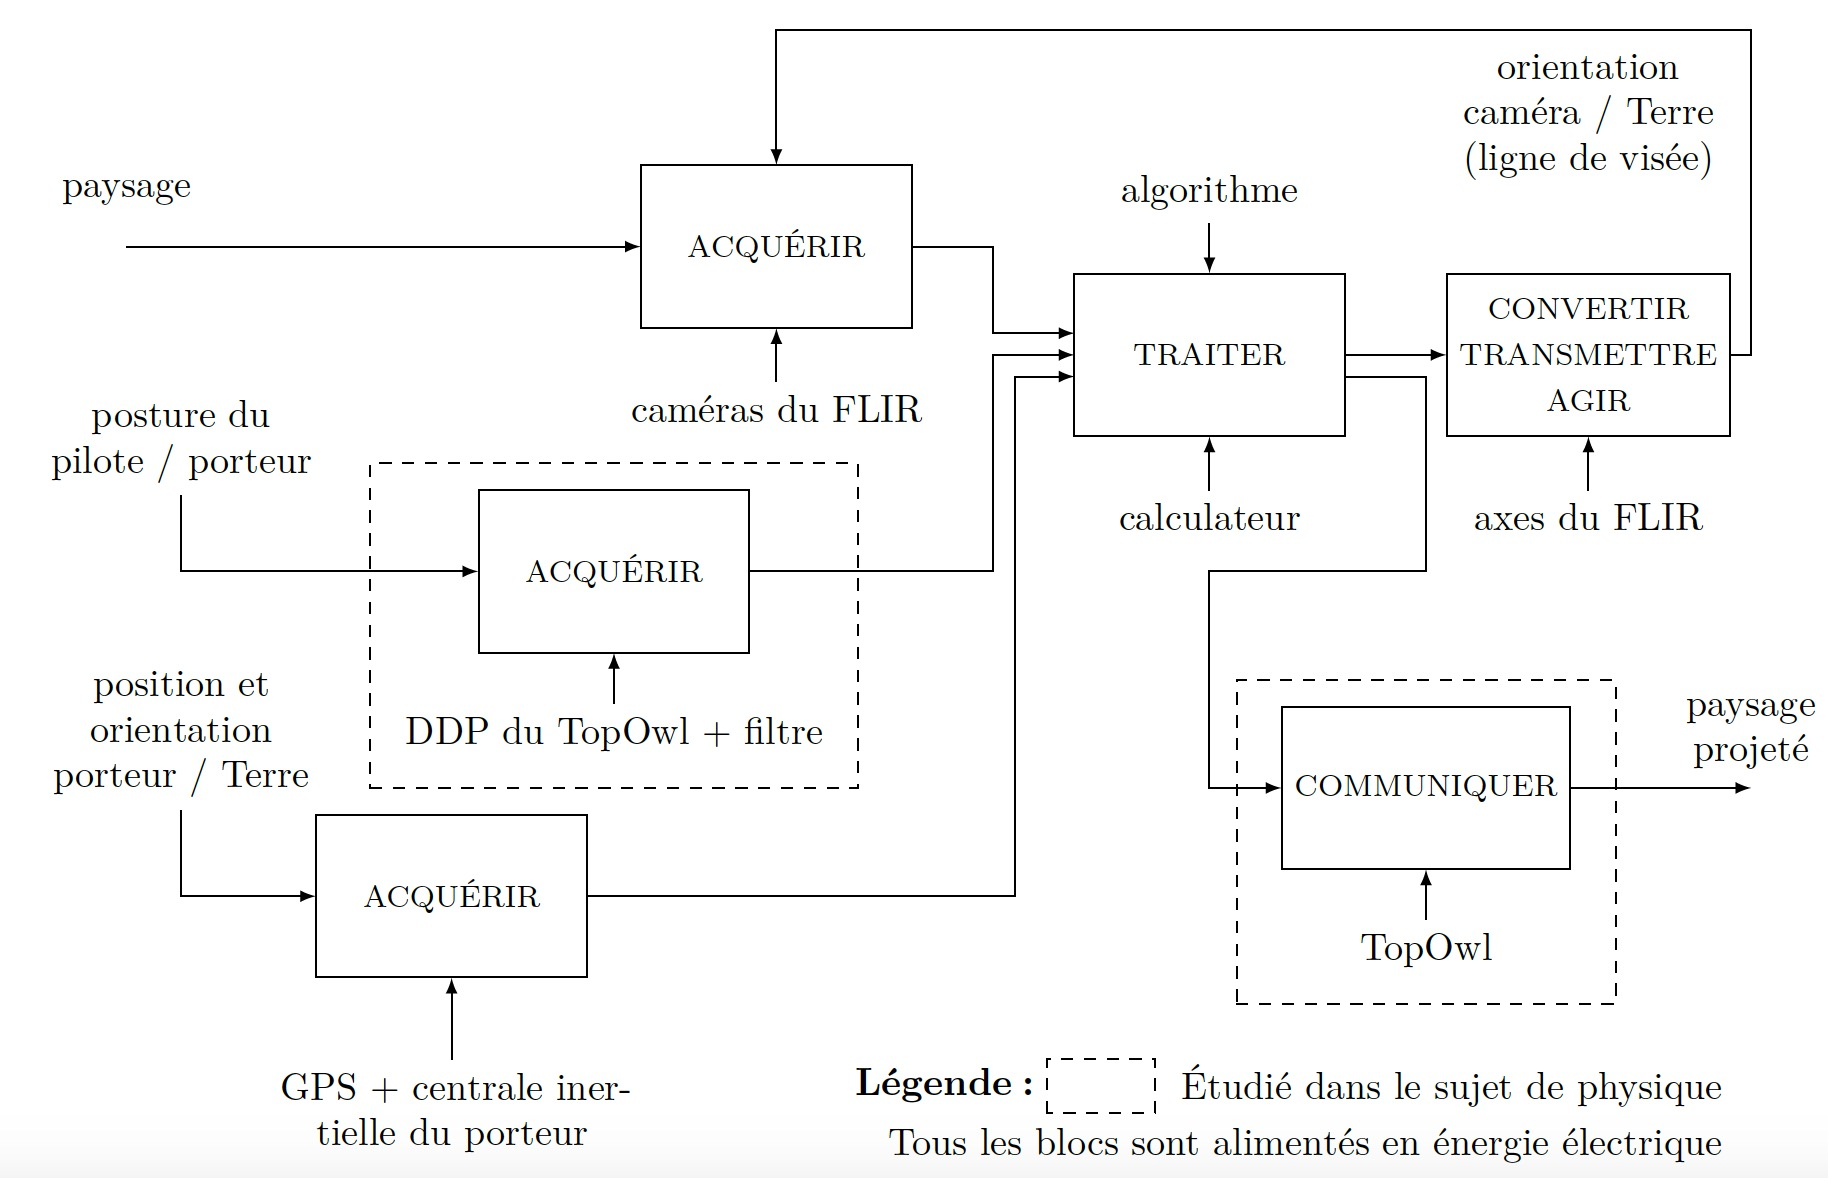
\includegraphics[width=0.9\textwidth]{chaine_fonctionnelle3.jpg}
\caption{Description structuro-fonctionnelle du système de vision en réalité augmentée \label{chaine_fonctionnelle}}
\end{center}
\end{figure}

\question{À l'aide de la description structuro-fonctionnelle de la figure \ref{chaine_fonctionnelle}, déterminer littéralement et numériquement
en fonction des données précédentes le temps maximal disponible pour orienter les caméras du FLIR, noté
$t_{disponible}$, qui permet de vérifier le troisième critère de l'exigence 1.1.}

\begin{figure}[!htb]
\begin{center}
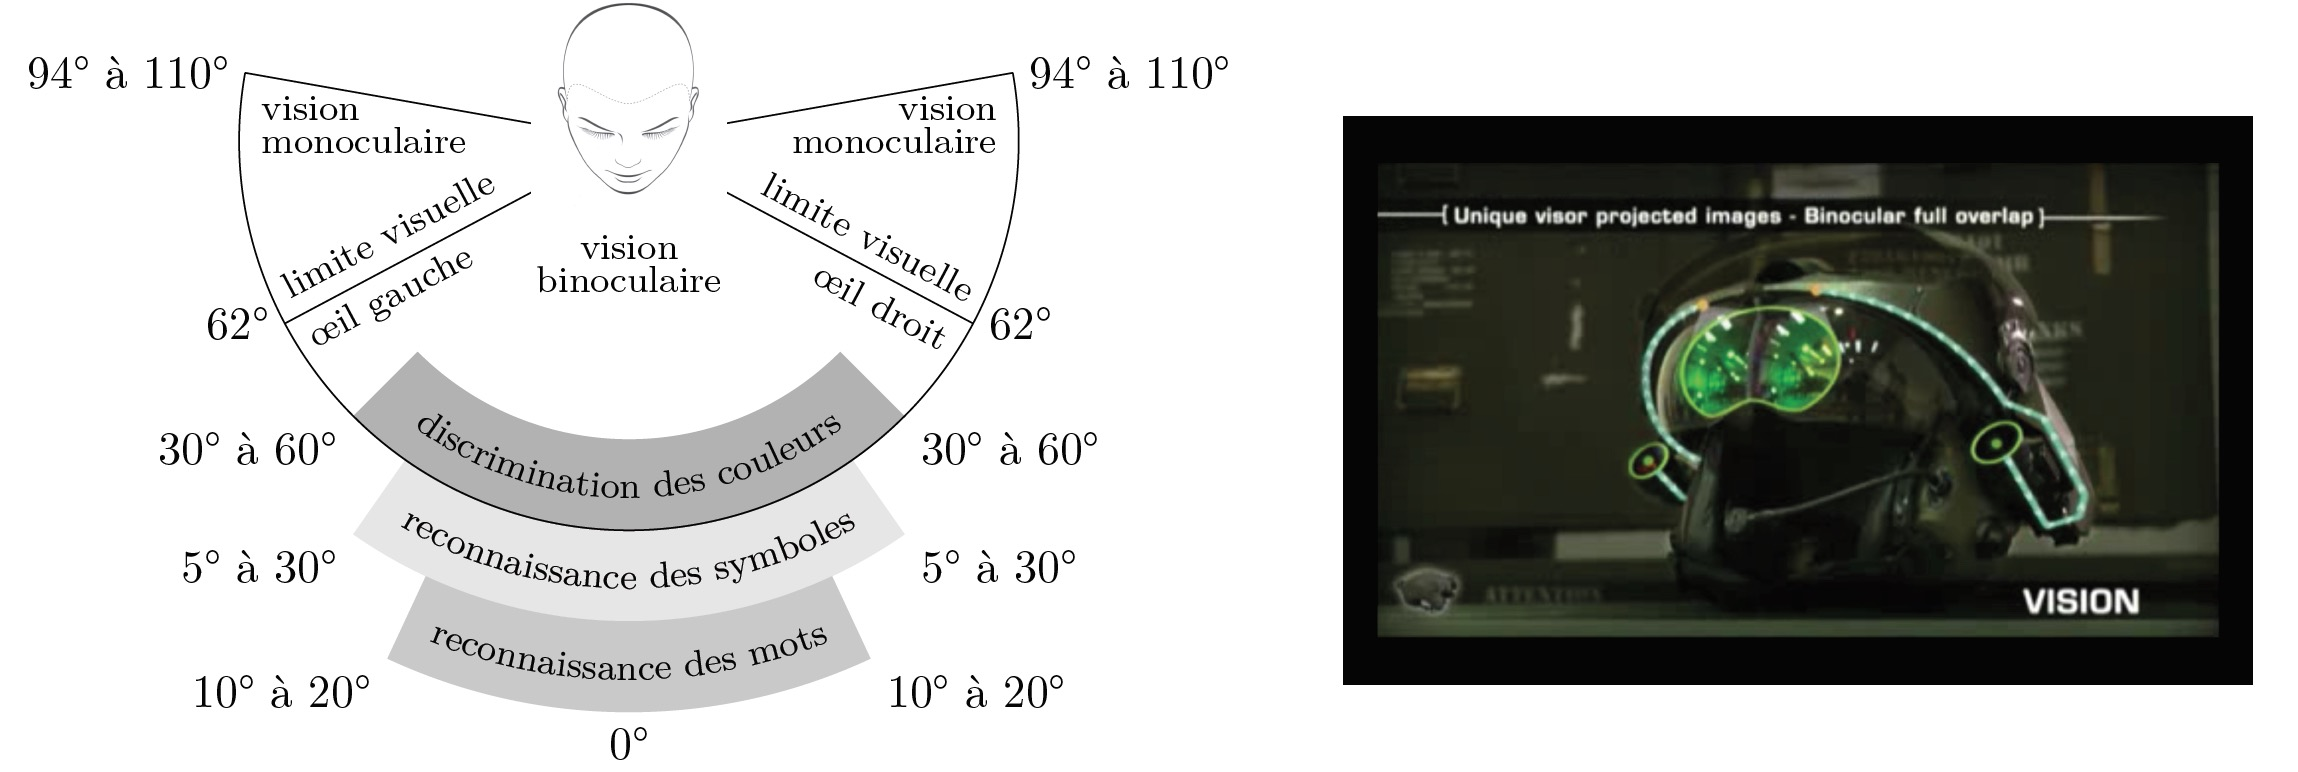
\includegraphics[width=0.9\textwidth]{figure6.jpg}
\caption{Champ de vision humain et projection des deux images sur la visière \label{figure6}}
\end{center}
\end{figure}

Le format choisi correspond à une image rectangulaire de 1024 pixels de large et 768 pixels de haut. Cette image
est projetée deux fois sur la visière, une projection pour chaque oeil du pilote. Les deux projections se chevauchent
entièrement (Binocular full overlap). La visière se trouve à 5 cm des yeux du pilote et chaque image est projetée
de façon à occuper entièrement le champ de vision le plus large possible permettant la reconnaissance des mots.

\question{Calculer à partir des informations précédentes et de la figure \ref{figure6} la largeur d'un pixel (en mm) projeté sur
la visière. Conclure quant au respect du critère de résolution d'affichage de l'exigence 1.1.}

\question{Déterminer l'écart angulaire maximal admissible, exprimé en rad, entre la ligne de visée du pilote et la
ligne de visée des caméras qui permet de respecter le critère de précision de l'exigence 1.1.}


Afin de vérifier les performances du FLIR qui viennent d'être déterminées, et compte tenu de son niveau de
complexité élevé, il est nécessaire d'émettre et de valider des hypothèses simplificatrices de modélisation relatives
à son comportement.

\subsection{Architecture du FLIR et hypothèses de modélisation}\label{partie2}

\begin{obj}
Vérifier que le choix de l'architecture du FLIR permet de satisfaire les performances établies en partie \ref{partie1}.
Valider des hypothèses simplificatrices afin de pouvoir évaluer les performances du FLIR.
\end{obj}

\subsubsection{Description et validation de l'architecture du FLIR}

\begin{obj}
Valider le choix de l'architecture du FLIR.
\end{obj}

Le FLIR, fixé au porteur, est constitué :
\begin{itemize}
\item d'un axe motorisé d'\textit{azimut} orientable en rotation par rapport au porteur autour de l'axe $\axe{P}{\vect{z_p}}$ ;
\item d'un ensemble de caméras, appelé \textit{charge}, encastré sur un \textit{axe motorisé d'élévation} orientable en rotation
par rapport à l'axe motorisé d'azimut autour de l'axe $\axe{P}{\vect{y_e}}$.
\end{itemize}

Le modèle cinématique du FLIR et son paramétrage sont donnés sur la figure \ref{figure7}.

\begin{figure}[!htb]
\begin{center}
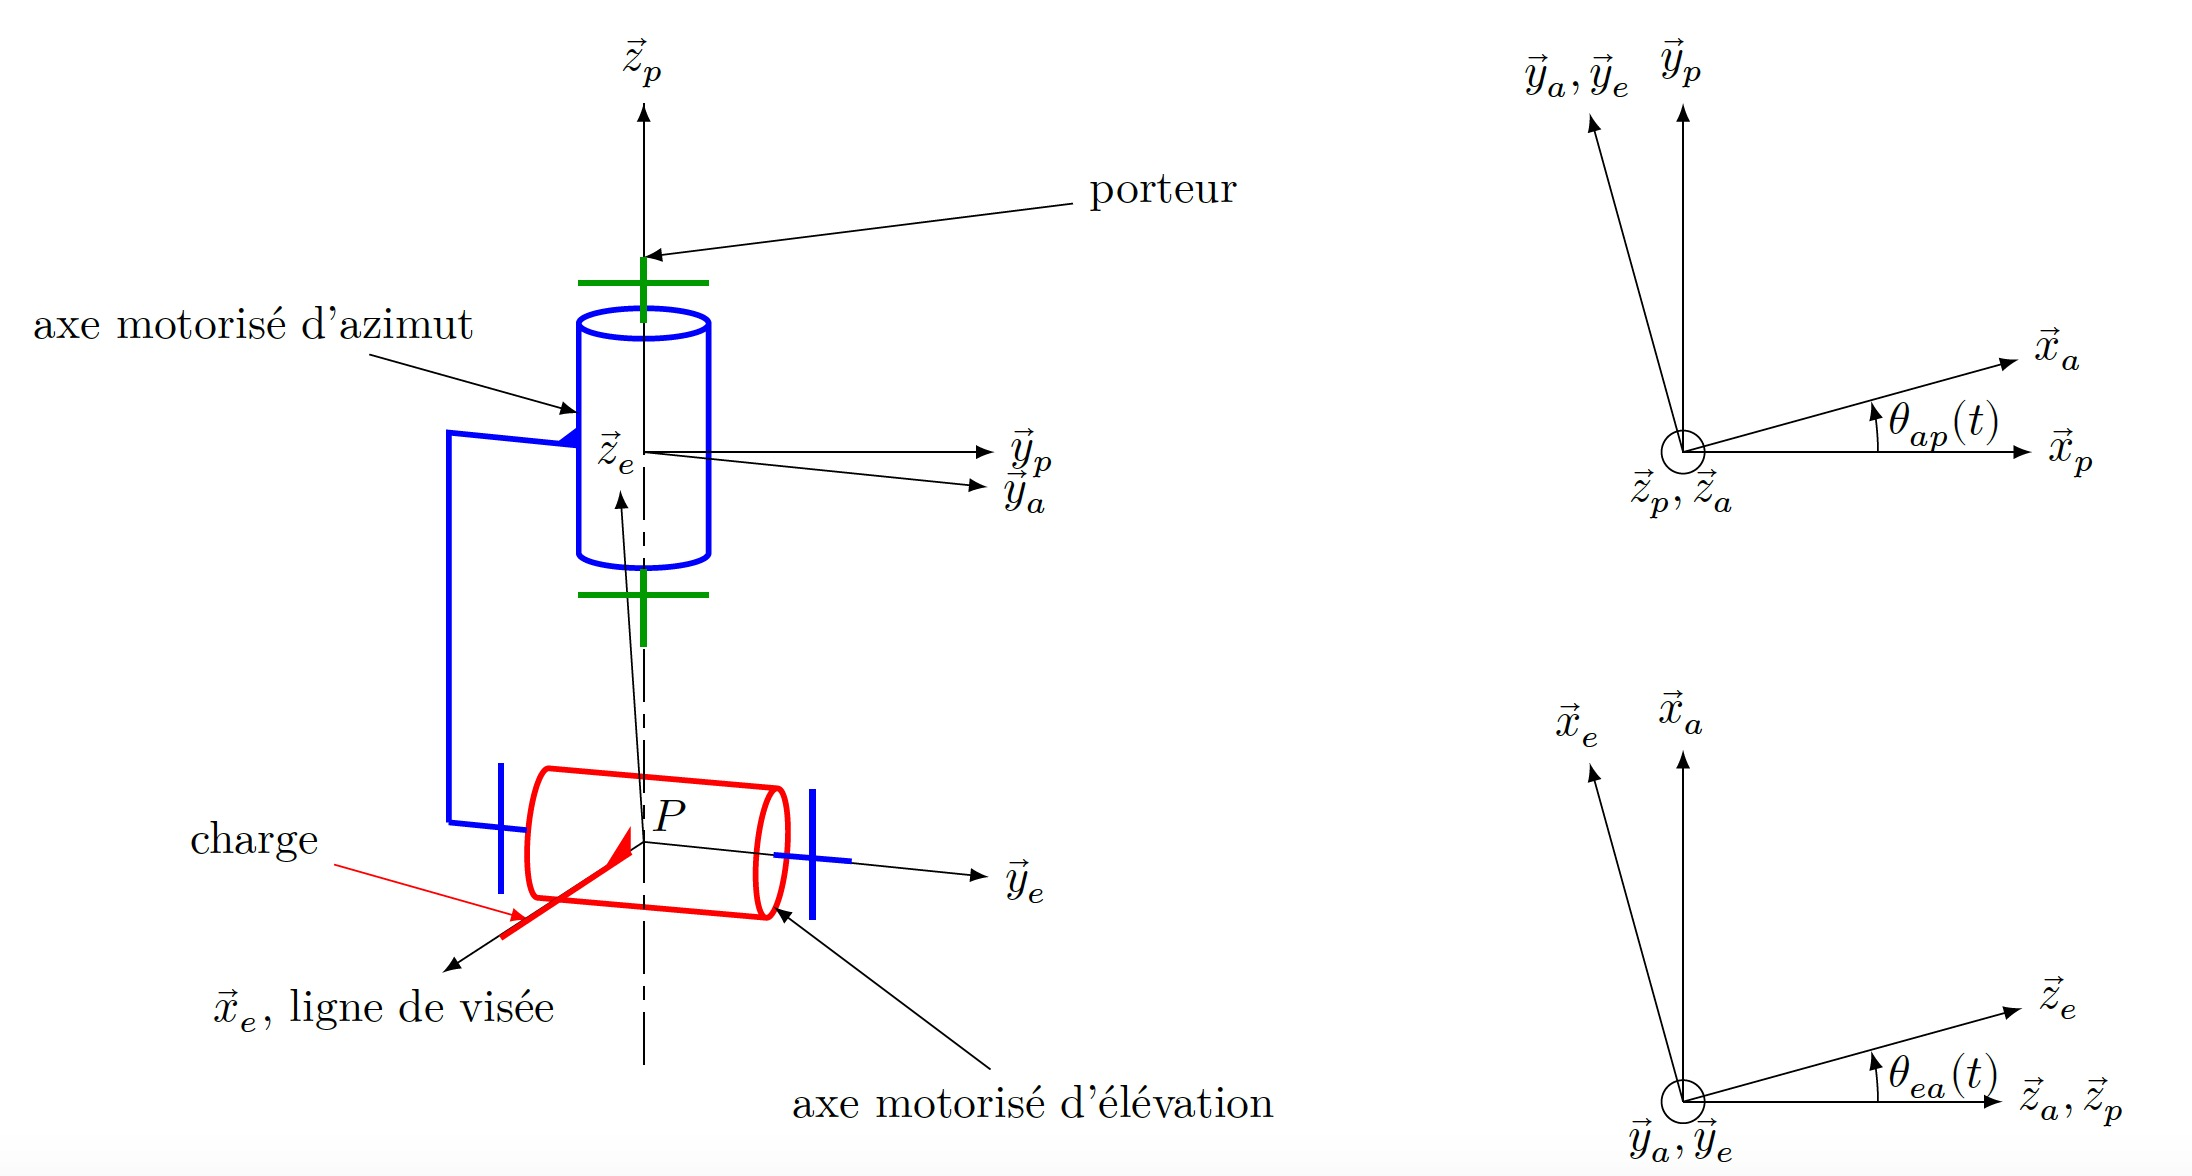
\includegraphics[width=0.9\textwidth]{figure7.jpg}
\caption{Modèle cinématique global paramétré du FLIR, motorisations enlevées \label{figure7}}
\end{center}
\end{figure}

Les repères associés aux solides sont les suivants :
\begin{itemize}
\item $R_a\quadruplet{P}{\vect{x_a}}{\vect{y_a}}{\vect{z_a}}$ pour l'axe motorisé d'azimut ;
\item $R_e\quadruplet{P}{\vect{x_e}}{\vect{y_e}}{\vect{z_e}}$ pour l'ensemble $\left\{\text{axe motorisé d'élévation, charge}\right\}$ dont la ligne de visée est portée par $\vect{x}_e$ ;
\item $R_p\quadruplet{P}{\vect{x_p}}{\vect{y_p}}{\vect{z_p}}$ pour le porteur ;
\item $R_0\quadruplet{P}{\vect{x_0}}{\vect{y_0}}{\vect{z_0}}$ référentiel terrestre non géocentrique, placé à la surface de la Terre au voisinage du porteur avec $\vect{z}_0$ vertical ascendant.
\end{itemize}

Dans la suite du sujet, le référentiel \textbf{$R_0$} est considéré comme galiléen.

\begin{figure}[!htb]
\begin{center}
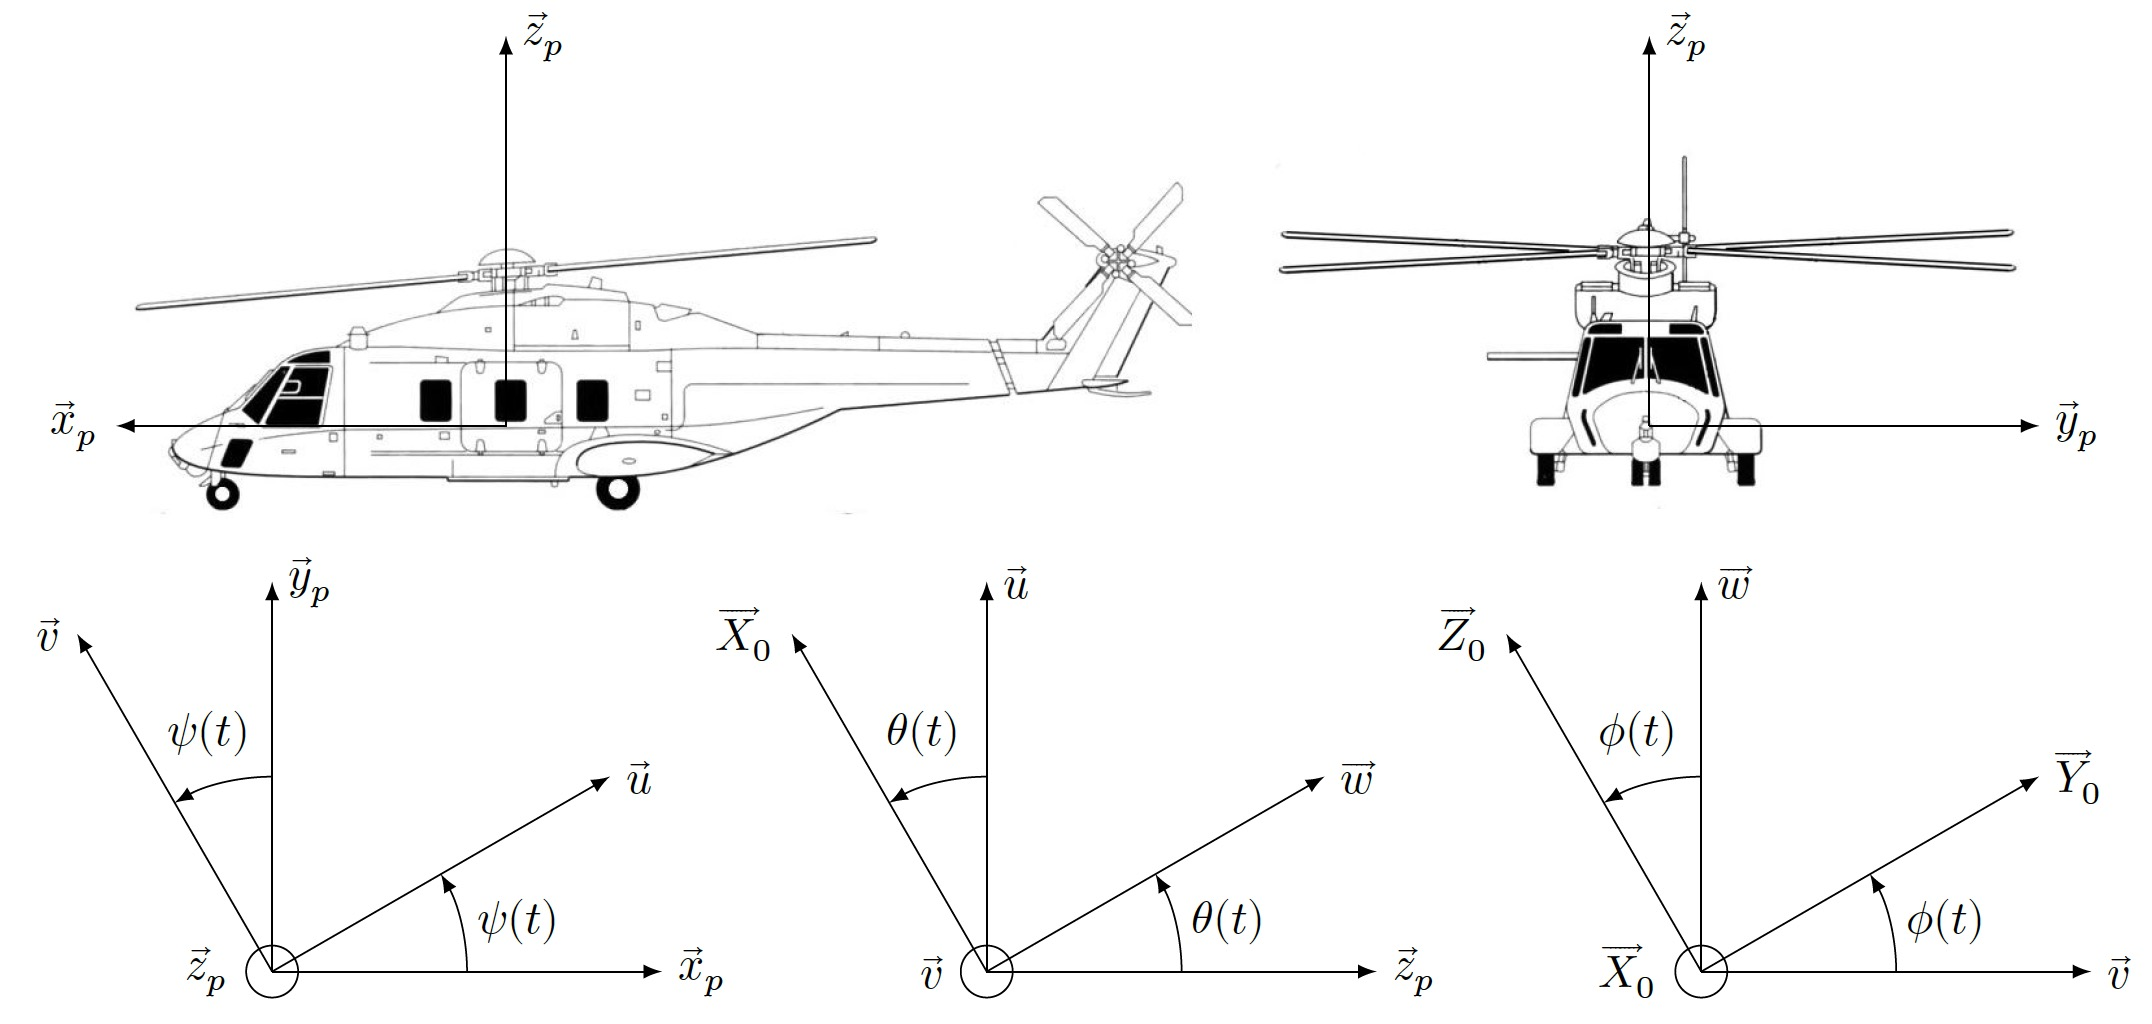
\includegraphics[width=0.9\textwidth]{figure8.jpg}
\caption{Porteur NH90 et son orientation par rapport au référentiel terrestre \label{figure8}}
\end{center}
\end{figure}

Le passage du référentiel terrestre $R_0$ au repère du porteur $R_p$ se fait par l'intermédiaire des trois angles de
Cardan définis sur la figure 8, avec :
\begin{itemize}
\item $\phi(t)$ l'angle de roulis ;
\item $\theta(t)$ l'angle de tangage ;
\item $\psi(t)$ l'angle de lacet.
\end{itemize}

\question{Déterminer le torseur cinématique en $P$ , exprimé dans la base $\base{\vect{x_a}}{\vect{y_a}}{\vect{z_a}}$ de la liaison équivalente
entre le porteur et la charge. En déduire la nature de cette liaison équivalente et préciser ses caractéristiques
géométriques.}

Dans un cas d'utilisation normal, la liaison cinématique entre la tête du pilote et le cockpit est assimilable à une
liaison sphérique dont le centre se trouve au milieu de la nuque. Or, le pilote doit avoir une image cohérente à
sa vision quelle que soit l'orientation de sa tête par rapport au porteur.

\question{Afin de pouvoir valider la solution technique retenue pour la structure cinématique à deux axes orthogonaux
motorisés du FLIR, comparer les mobilités du FLIR et celles de la tête du pilote par rapport au porteur
et expliquer quel doit être un des rôles de l'algorithme implanté dans le calculateur.}

\subsection{Hypothèses simplificatrices}

\begin{obj}
Valider les hypothèses simplificatrices suivantes :
\begin{itemize}
\item la commande de l'axe motorisé d'azimut est indépendante des mouvements de l'axe motorisé
d'élévation ;
\item  les effets aérodynamiques et la variation de position du centre d'inertie de la charge n'influent pas
sur les performances du FLIR.
\end{itemize}

\end{obj}

\subsubsection{Limitation de l'étude à l'axe motorisé d'élévation}

La charge mue par l'axe motorisé d'élévation est essentiellement constituée de caméras et de cartes électroniques
associées. Les ingénieurs ont choisi de disposer ces composants de telle sorte que la répartition des masses de
cette charge s'approche au mieux de celle d'un cylindre plein et homogène d'axe $\axe{P}{\vect{y_e}}$ de la figure \ref{figure7}.

\question{Justifier que le choix de la répartition des composants de la charge, dans le cas du mouvement simultané
des deux axes motorisés décrits sur la figure \ref{figure7}, permet de commander l'axe d'azimut indépendamment de l'axe
motorisé d'élévation.}

Les résultats d'essais en vol montrent que l'axe qui subit le plus de perturbations est l'axe motorisé d'élévation.
Les commandes des axes d'élévation et d'azimut étant indépendantes l'une de l'autre, la suite de l'étude se
limitera uniquement à l'axe motorisé d'élévation.

\subsubsection{Rigidité de la structure à double étage de l'axe motorisé d'élévation et influence des
perturbations aérodynamiques}

\begin{figure}[!htb]
\begin{center}
\begin{minipage}{0.45\textwidth}
Afin de limiter l'influence des vibrations du porteur sur la
ligne de visée et augmenter la précision de son orientation,
les ingénieurs ont choisi de décomposer l'axe motorisé
d'élévation en deux étages (voir figures \ref{fig9} et \ref{figure10}).
Le premier étage, appelé étage gros d'élévation ($ge$), est
en prise directe avec l'air et est donc soumis aux effets
aérodynamiques lors des mouvements du porteur. L'étage
gros d'élévation est lui même en liaison pivot, d'axe $\axe{P}{\vect{y_e}}$,
avec l'axe motorisé d'azimut.
\end{minipage}
\begin{minipage}{0.45\textwidth}
\begin{center}
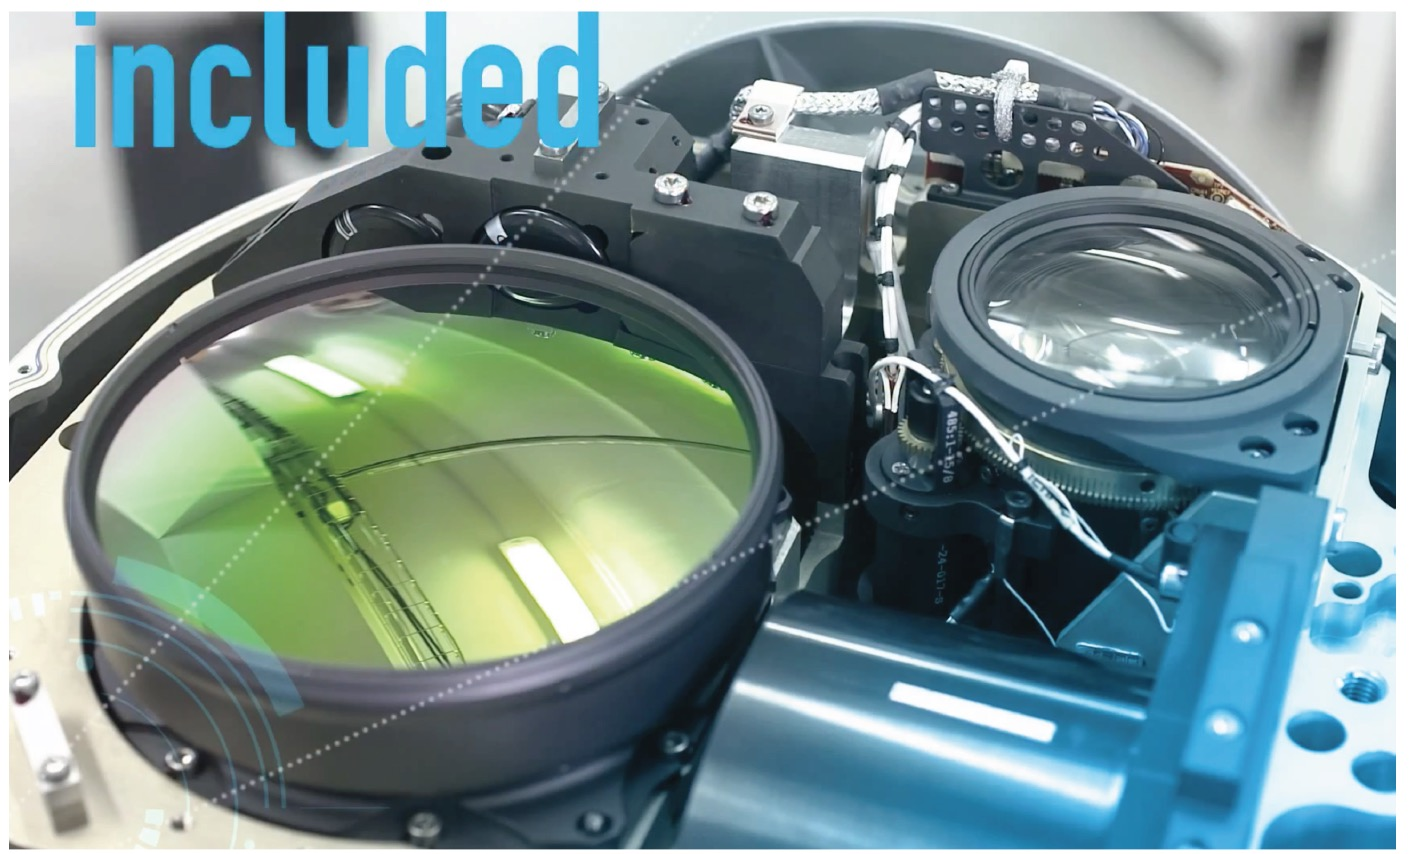
\includegraphics[width=0.8\textwidth]{figure9.jpg}
\caption{Intérieur du FLIR, vue des optiques des
caméras liées à l'étage fin d?élévation\label{fig9}}
\end{center}
\end{minipage}
\end{center}
\end{figure}

%\FloatBarrier

Le second, appelé étage fin d'élévation ($fe$), est protégé
des effets aérodynamiques grâce au carter sphérique
solidaire de l'étage gros. Cet étage est en liaison pivot,
d'axe $\axe{P}{\vect{y_e}}$, avec l'étage gros d'élévation. L'inertie des
éléments déplacés par l'étage fin d'élévation est plus faible
que celle de l'étage gros d'élévation et les choix de guidage
et de motorisation permettent d'atteindre des accélérations
et des vitesses élevées. Cependant, l'amplitude du mouvement de l'étage fin est limitée.

\begin{figure}[!htb]
\begin{center}
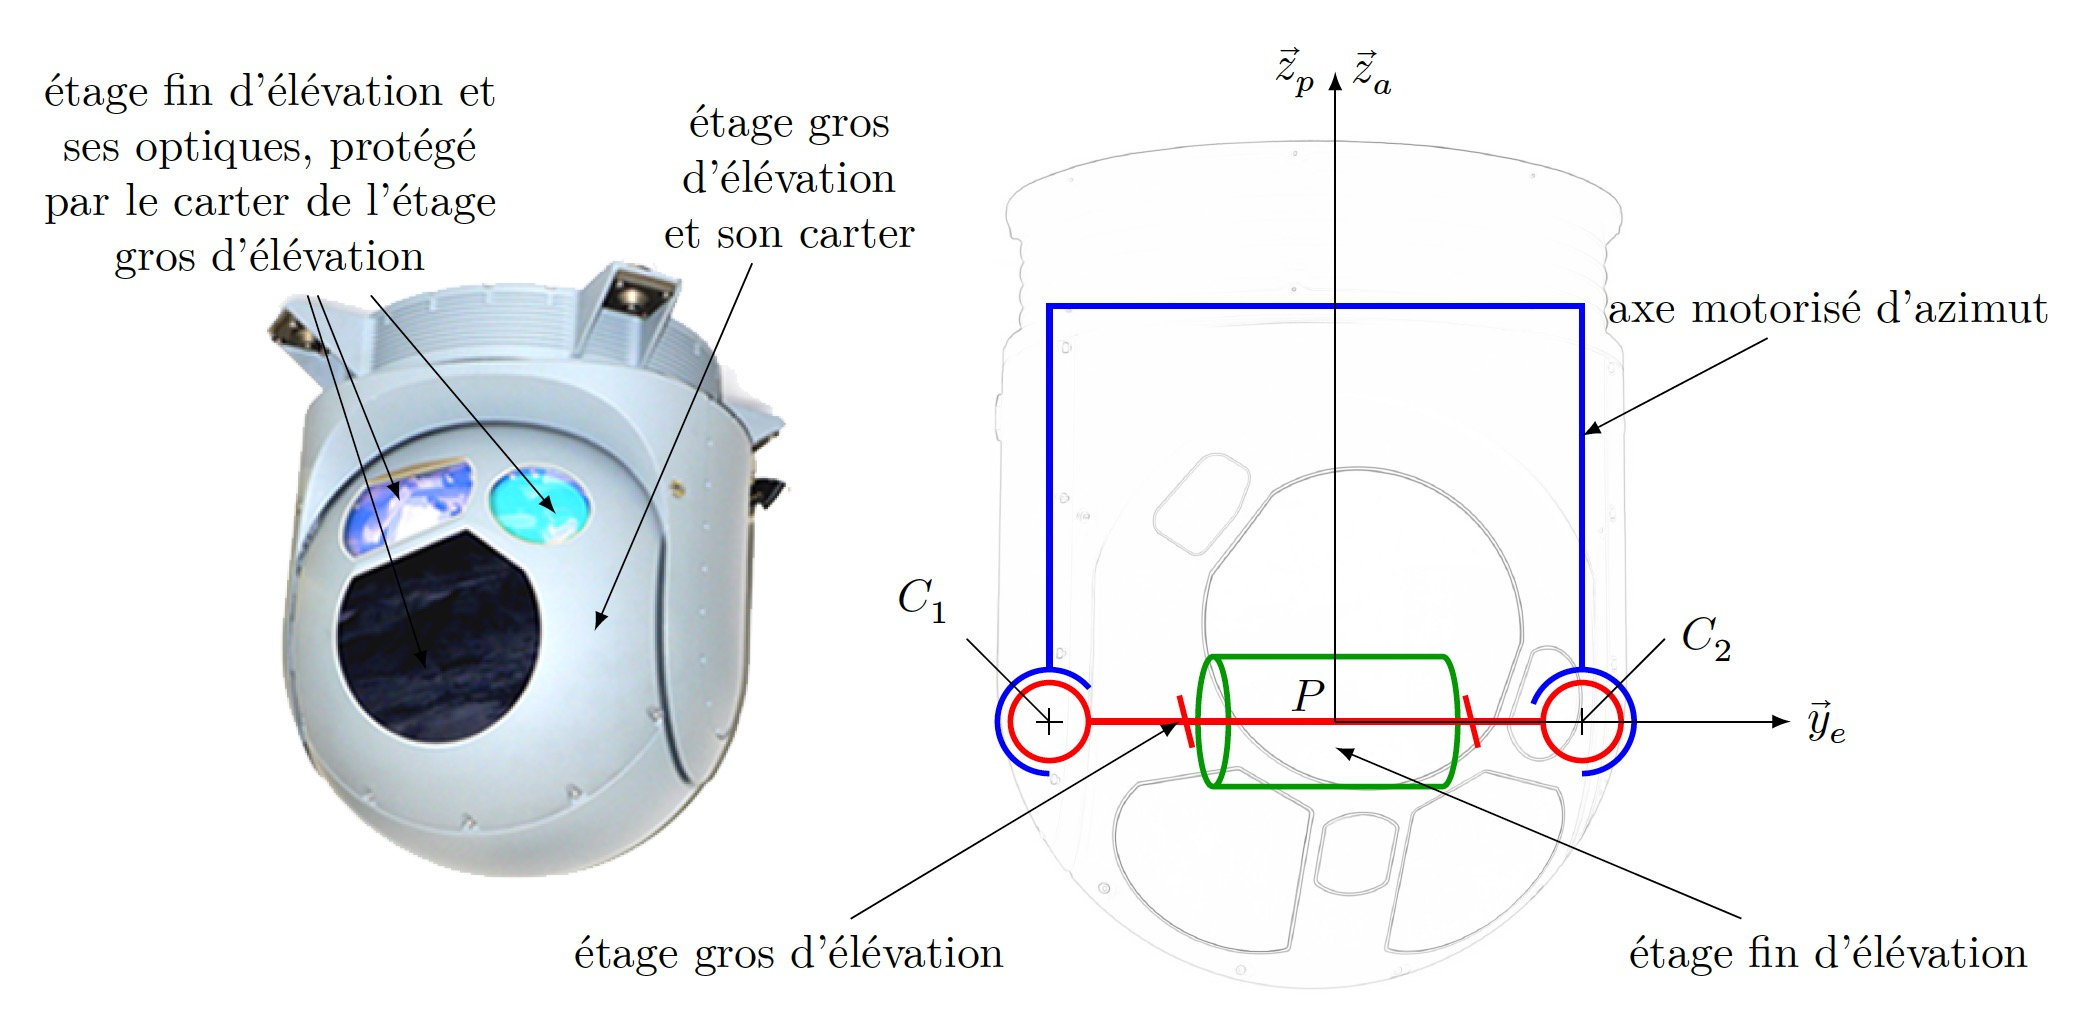
\includegraphics[width=0.9\textwidth]{figure10.jpg}
\caption{FLIR et modèle cinématique de l'axe motorisé d'élévation \label{figure10}}
\end{center}
\end{figure}

Le guidage en rotation entre l'étage gros d'élévation et l'axe motorisé d'azimut est réalisé à l'aide de deux
composants à éléments roulants modélisables par des liaisons sphériques de centre $C_1$ et $C_2$.

\begin{figure}[!htb]
\begin{center}
\begin{minipage}{0.45\textwidth}
\question{(Réservée aux 5/2) À l'aide de la figure \ref{figure10}, déterminer le degré
d'hyperstatisme du modèle du guidage en rotation
entre l'axe motorisé d'azimut et l'étage gros d'élévation.
Lister deux avantages et un inconvénient
de ce guidage, puis conclure quant à sa pertinence
vis-à-vis de la précision de l'orientation de la ligne
de visée souhaitée.}

Le montage de l'étage gros d'élévation sur l'axe motorisé
d'azimut induit des efforts axiaux égaux, opposés
et dirigés suivant $\vect{y}_e$, dans les liaisons de centre
$C_1$ et $C_2$. Ces efforts, appelés précharge, sont réglables
au montage en jouant sur la différence de distance
entre les points $C_1$ et $C_2$ prise d'une part, sur
l'axe motorisé d'azimut et, d'autre part, sur l'étage
gros d'élévation.
\end{minipage}
\begin{minipage}{0.45\textwidth}
\begin{center}
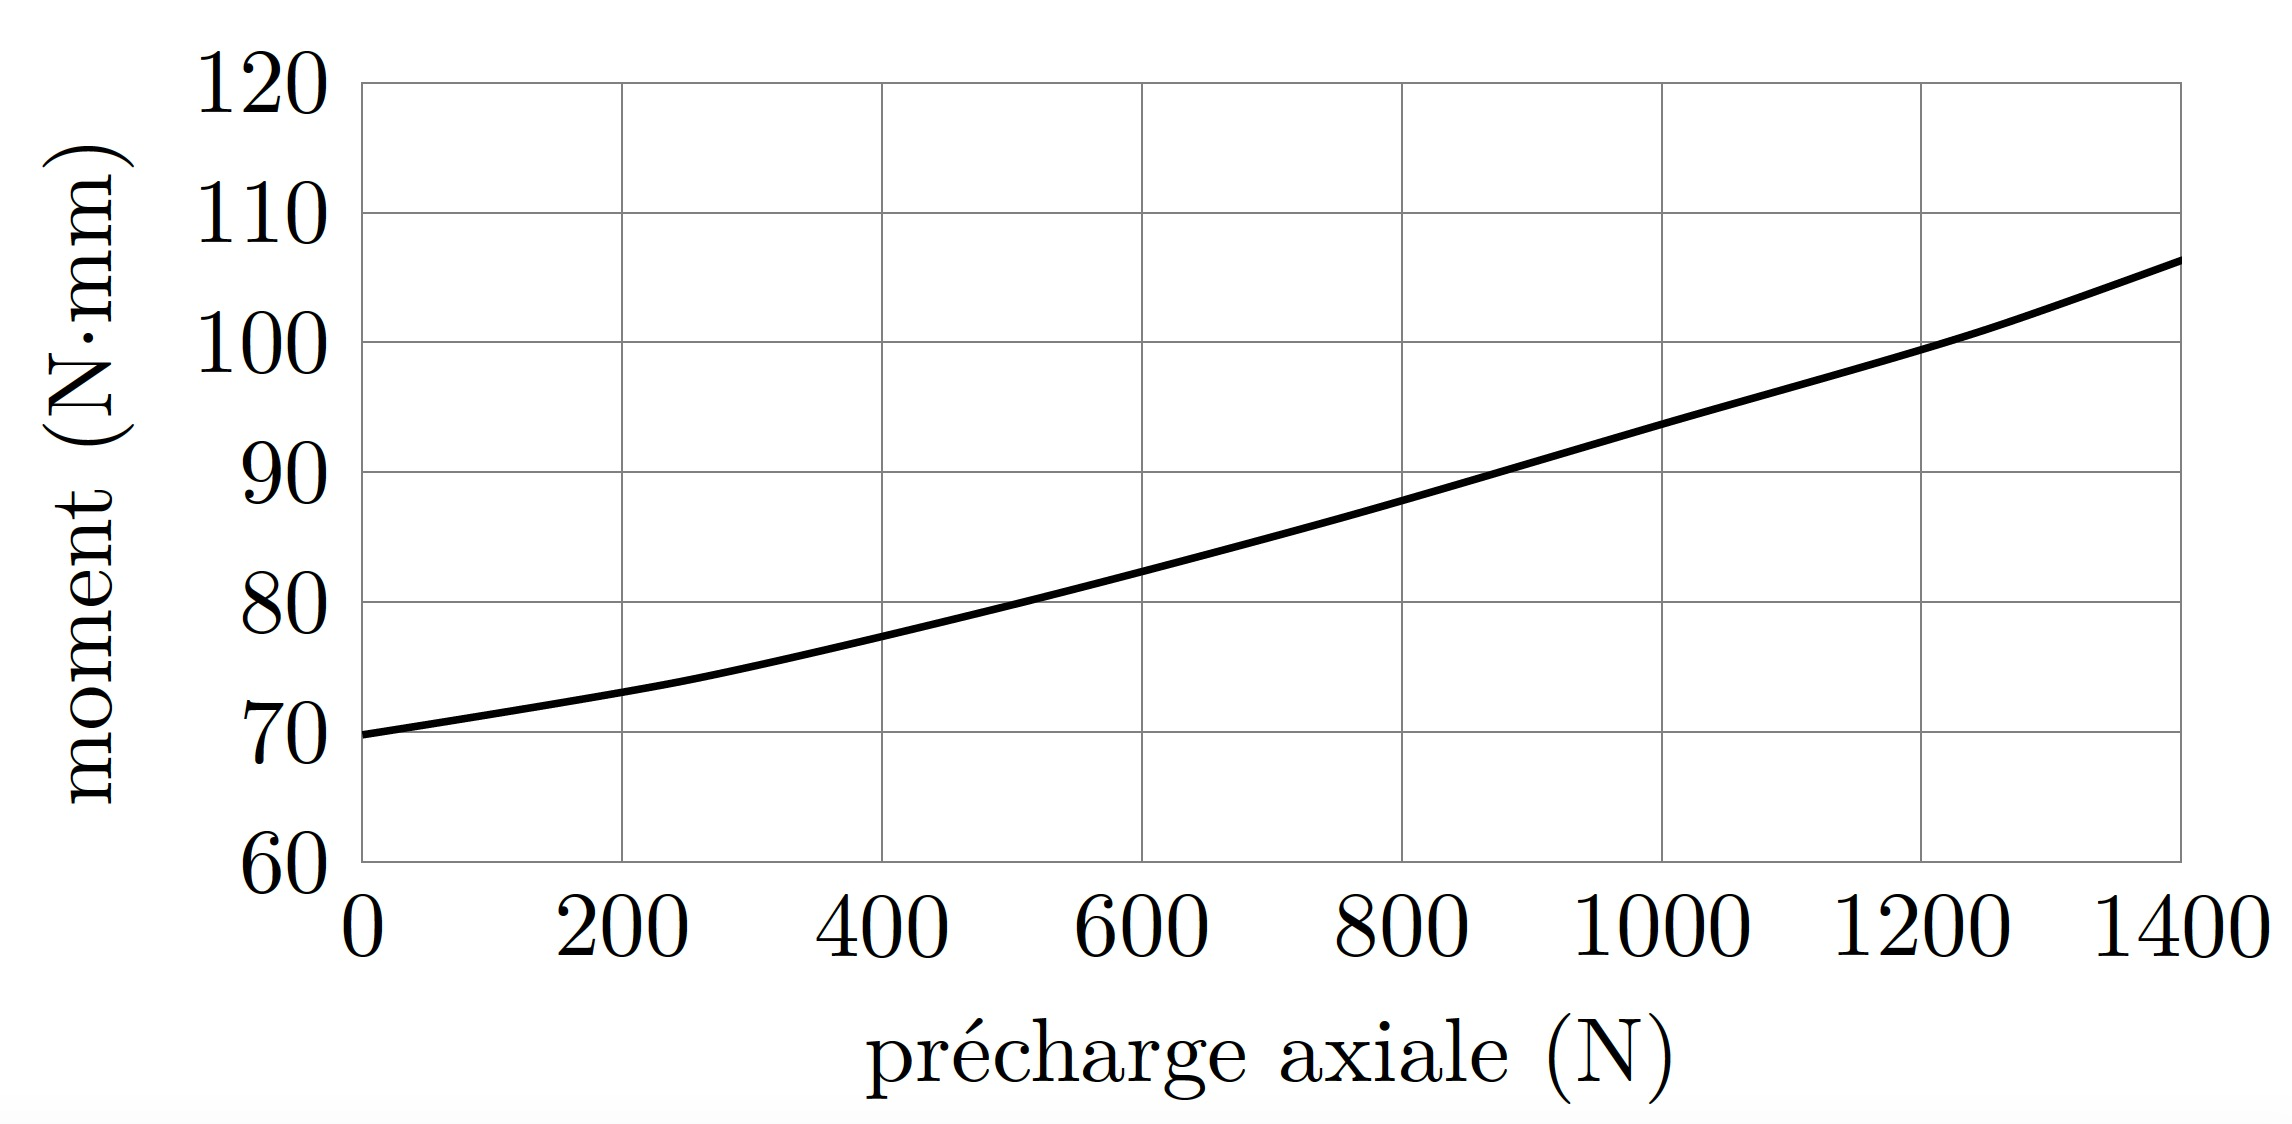
\includegraphics[width=0.9\textwidth]{figure11.jpg}
\caption{Moment de frottement sec d'un seul composant
à éléments roulants du guidage en rotation de l'étage
gros d'élévation par rapport à l'axe motorisé d'azimut, en
fonction de la précharge axiale (source : SKF)\label{fig11}}
\end{center}
\end{minipage}
\end{center}
\end{figure}
%\FloatBarrier

Lors des conditions de vol les plus sévères, le couple exercé par les effets aérodynamiques sur le carter de l'étage
gros d'élévation a été mesuré à $0,18 N\cdot m$.

\question{À l'aide de l'abaque donné figure \ref{fig11}, déterminer une valeur de réglage pertinente de la précharge du
guidage en rotation de l'étage gros d'élévation par rapport à l'axe motorisé d'azimut.}

%\FloatBarrier
\subsubsection{Influence du déport de masse lié à la variation de position des optiques}

Le déplacement des optiques (zoom) en translation rectiligne suivant $\vect{x}_e$ par rapport à l'étage fin d'élévation
rend la géométrie de ce dernier variable et son centre d'inertie ne se situe pas exactement sur l'axe de rotation
$\axe{P}{\vect{y_e}}$ de l'étage fin d'élévation par rapport à l'étage gros d'élévation.
L'étage fin d'élévation est modélisé par l'ensemble des deux solides suivants (voir figure \ref{figure12}) :
\begin{itemize}
\item un disque plein et homogène d'axe $\axe{P_0}{\vect{x_e}}$ de masse $m_o$, de rayon $r_o$ et de centre de gravité $P_o$, modélisant les optiques mobiles de l'étage fin d'élévation ;
\item un cylindre plein et homogène d'axe $\axe{P}{\vect{y_e}}$ de masse $m_{cyl}$, de rayon $r_{cyl}$, de hauteur $h_{cyl}$ et de centre de gravité $P$, modélisant le reste des éléments de l'étage fin d'élévation.
\end{itemize}

Dans la suite, ces deux solides sont supposés être en liaison complète, c'est-à-dire que la distance $d$, telle que $\vect{PP_0}=d\vect{x}_e$ est constante.

\begin{figure}[!htb]
\begin{center}
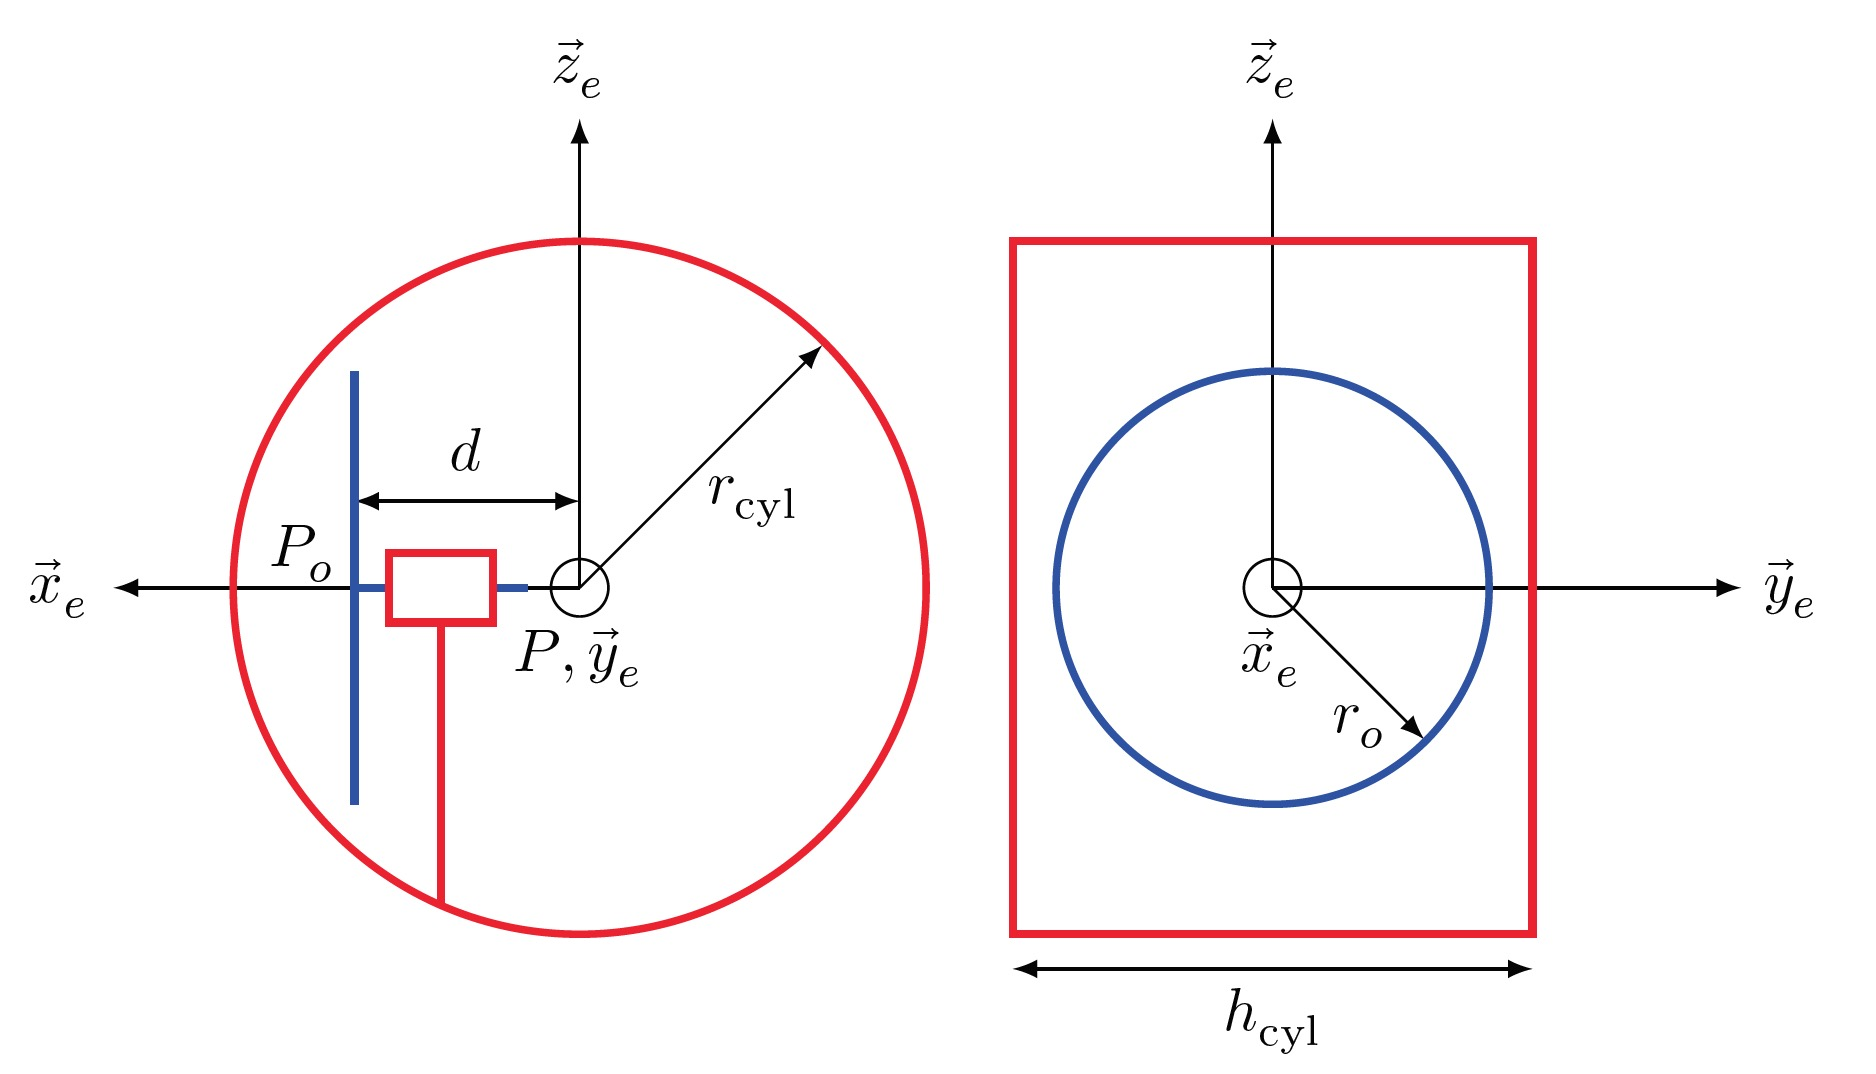
\includegraphics[width=0.6\textwidth]{figure12.jpg}
\caption{Modélisation de la géométrie des masses de l'étage fin d'élévation \label{figure12}}
\end{center}
\end{figure}

\begin{itemize}
\item L'opérateur d'inertie du cylindre plein, noté $cyl$, est de la forme suivante :
$
\overline{\overline{I}}_P(cyl)=
\left(
\begin{array}{ccc}
A_{cyl} & 0 & 0 \\ 
0 & B_{cyl} & 0 \\ 
0 & 0 & A_{cyl}
\end{array}
\right)_{\base{\vect{x_e}}{\vect{y_e}}{\vect{z_e}}} 
$
\item L'opérateur d'inertie des optiques, noté $o$, est de la forme suivante :
$
\overline{\overline{I}}_{P_o}(o)=
\left(
\begin{array}{ccc}
A_{o} & 0 & 0 \\ 
0 & B_{o} & 0 \\ 
0 & 0 & B_{o}
\end{array}
\right)_{\base{\vect{x_e}}{\vect{y_e}}{\vect{z_e}}} 
$
\item L'étage fin d'élévation est noté $f_e$, sa masse est égale à $m_{fe}=m_{cyl}+m_o$, son centre d'inertie est noté $G_{fe}$.
\end{itemize}

\question{Déterminer littéralement l'opérateur d'inertie $\overline{\overline{I}}_P(fe)$ de l'étage fin d'élévation en fonction de $A_{cyl}$, $B_{cyl}$, $A_o$, $B_o$, $d$ et $m_o$ dans le repère $R_e$, puis exprimer le vecteur $\vect{PG_{fe}}=\lambda \cdot \vect{x}_e$ dans le repère $R_e$ en fonction de $m_{cyl}$, $m_o$ et $d$.}

Des mesures à bord du NH90 ont montré que la phase de vol la plus pénalisante, c'est-à-dire celle qui perturbe
le plus la ligne de visée du FLIR, est l'ascension verticale du porteur. Dans cette phase, il est possible d'effectuer
les hypothèses suivantes :
\begin{itemize}
\item les angles $\psi(t)$, $\theta(t)$ et $\phi(t)$ sont constants et nuls ;
\item $\theta_{ap}(t)=0$ ;
\item $\vect{z}_p=\vect{z}_a=\vect{z}_0$ vertical ascendant, $\vect{y}_p=\vect{y}_a=\vect{y}_0$ et $\vect{x}_p=\vect{x}_a=\vect{x}_0$;
\item l'étage fin d'élévation est en mouvement par rapport à l'étage gros d'élévation ;
\item la ligne de visée est définie par l'orientation $\theta_{eo}(t)$ de l'étage fin d'élévation par rapport à $R_0$. Dans cette
étude, $\theta_{e0}(t)=\theta_{ea}(t)$;
\item $R_0$ est galiléen ;
\item le couple moteur sur l'étage fin d'élévation est noté $C_m(t)$ ;
\item la liaison pivot entre l'étage fin d'élévation et l'étage gros d'élévation est supposée parfaite.
\end{itemize}

La vitesse d'ascension verticale du porteur est notée $\vect{V}(P\in porteur/R_0)=v(t)\cdot \vect{z}_0$ et son accélération est notée $\vect{\Gamma}(P\in porteur/R_0)=\gamma(t)\cdot \vect{z}_0$.

Les dérivées d'un paramètre $x(t)$ par rapport au temps seront notées : $\dot{x}(t)=\frac{dx(t)}{dt}$ et $\ddot{x}(t)=\frac{d^2x(t)}{dt^2}$. 

\question{Montrer que $\vect{V}(G_{fe}\in fe/R_0)$, vecteur vitesse du point $G_{fe}$, centre d'inertie de l'étage fin d'élévation dans son mouvement par rapport à $R_0$, peut s'écrire sous la forme : $\vect{V}(G_{fe}\in fe/R_0)=a(t)\cdot \vect{z}_0+b(t)\cdot \vect{z}_e$. L'exprimer alors en fonction de $v(t)$, $m_{cyl}$, $m_o$, $d$, $\theta_{eo}(t)$ et $\dot{\theta}_{eo}(t)$.}


\question{Déterminer l'accélération $\vect{\Gamma\left( G_{\text{fe}},fe/R_0 \right)}$}


\question{Isoler $fe$ et faire les bilan des actions mécaniques en écrivant tous les torseurs en $P$}




\question{Énoncer le théorème du moment dynamique appliqué à $fe$ en $P$ sans développer le calcul.}


\question{Donner la relation liant le moment dynamique en $P$ ($\vect{\delta\left( P,fe/R_0 \right)}$) à celui en $G_{fe}$ ($\vect{\delta\left( G_{\text{fe}},fe/R_0 \right)}$)}


\question{Déterminer le moment cinétique $\vect{\sigma\left( G_{\text{fe}},fe/R_0 \right)}$ puis le moment dynamique au même point : \(\vect{\delta\left( G_{\text{fe}},fe/R_0 \right)}$}


\question{En déduire le moment dynamique : $\vect{\delta\left( P,fe/R_0 \right)}$}



\question{En déduire l'équation différentielle régissant le mouvement de l'étage fin d'élévation par rapport
au référentiel galiléen $R_0$.}

Les valeurs numériques suivantes sont données : $m_o = 1,4 kg$ ; $d= 0,01 m$ ; $\vert \gamma(t)\vert_{\text{MAXI NH90}} = 1,8 g$, avec $g\approx  9,81 m\cdot s^{-2}$.

Les couples perturbateurs voisins du dixième de la valeur du couple moteur maximal seront négligés vis-à-vis
de ce dernier lors de la conception de la commande. Pour l'étage fin d'élévation, le couple moteur maximal est
voisin de $3 N\cdot m$.

\question{Dans la phase de vol étudiée, donner sous forme littérale l'expression du couple de perturbation issu du
déport de masse $d$, noté $C_{pert}$. Calculer la valeur numérique maximale de $C_{pert}$, notée $C_{\text{pertMAXI}}$, dans le cas le plus défavorable. Conclure sur la pertinence de la prise en compte de cette perturbation pour la conception de
la commande de l'étage fin d'élévation.}

\subsection{Conception de la commande de l'axe motorisé d'élévation à partir
des performances attendues et vérification des performances
simulées du FLIR}

\begin{obj}
Modéliser l'asservissement de l'axe motorisé d'élévation, concevoir sa commande puis vérifier ses performances
simulées vis-à-vis du cahier des charges donné sur le tableau \ref{tab2}.
\end{obj}

\begin{table}[!htb]
\begin{center}
\begin{tabular}{|p{0.3\textwidth}|p{0.3\textwidth}|p{0.3\textwidth}|}
\hline 
\textbf{Exigence} & \textbf{Critère} & \textbf{Valeur} \\ 
\hline 
1.4 Acquérir une image du paysage
extérieur suivant la ligne de visée
du pilote & Retard de trainage maximal de la
ligne de visée du FLIR & $40ms$ \\ 
\cline{2-3} 
& Précision angulaire de la ligne de
visée du FLIR & $680\mu rad$\\ 
\cline{2-3}  
 & Stabilité de la ligne de visée du
FLIR & Oscillations d'amplitude inférieure
à $340 \mu rad$ \\ 
\hline  
Être insensible aux perturbations
de l'air ambiant & Forme extérieure & Couple aérodynamique minimum\\ 
\hline
\end{tabular} 
\caption{Cahier des charges partiel du FLIR \label{tab2}}
\end{center}
\end{table}

%\FloatBarrier
\subsubsection{Modélisation de l'asservissement de l'étage fin d'élévation}

\begin{obj}
En s'appuyant sur les hypothèses validées en partie \ref{partie2}, compléter la modélisation de l'asservissement de
l'étage fin d'élévation et ajuster un correcteur qui lui permette d'atteindre les performances attendues.
\end{obj}

Un gyromètre est placé directement sur l'étage fin d'élévation et permet de mesurer $\omega_{fe0\text{ mes}}(t)$, taux de rotation de l'étage fin d'élévation par rapport au référentiel galiléen $R_0$. Les ingénieurs ont donc choisi d'asservir l'étage
fin d'élévation en vitesse angulaire afin d'utiliser directement la mesure du gyromètre.

La direction de la ligne de visée est paramétrée par rapport au référentiel galiléen $R_0$ par l'angle $\theta_{fe0}(t)=\theta_{e0}(t)$.

Sont donnés les éléments suivants :
\begin{itemize}
\item $\dot{\theta}_{fe0}(t)=\omega_{fe0}(t)=\vect{\Omega}(fe/R_0)\cdot \vect{y}_e$ où $\vect{\Omega}(fe/R_0)$ est le vecteur taux de rotation de l'étage fin d'élévation ($fe$) dans
son mouvement par rapport au référentiel terrestre $R_0$ ;
\item le comportement du gyromètre, placé directement sur l'étage fin d'élévation, peut être modélisé par un
premier ordre de gain unitaire et de bande passante à $-3 dB$ égale à $100 Hz$ ;
\item l'étage fin d'élévation ($f_e$) est actionné par un moteur électrique linéaire comme indiqué sur la figure\ref{figure14},
dont la tige est en liaison sphérique en $A$ avec l'étage fin d'élévation et le carter en liaison sphérique en $B$ avec l'étage gros d'élévation ;
\item l'isolement de la tige seule du moteur électrique linéaire permet de modéliser son action mécanique de liaison
en $A$ sur l'étage fin d'élévation par un glisseur au point $A$ de résultante $F_{mot}(t)\vect{u}$ ;
\item l'étage fin d'élévation ($fe$) est en liaison pivot d'axe $\axe{P}{\vect{y_e}}$ avec l'étage gros d'élévation ($ge$) ;
\item $\vect{AP}=r\cdot \vect{x}_e$ avec $r=10cm$ ;
\item $\lambda(t)$ paramètre la position de la tige par rapport au carter du moteur électrique linéaire tel que $\vect{BA}=\lambda(t)\cdot \vect{u}$.
\end{itemize}

Le choix de la motorisation de l'étage fin d'élévation permet d'atteindre des accélérations importantes mais
l'amplitude du mouvement de l'étage fin d'élévation ($fe$) par rapport à l'étage gros d'élévation ($ge$) est limitée
à l'intervalle $\left[-5^{\circ}, +5^{\circ}\right]$. Il est donc nécessaire d'orienter également l'étage gros d'élévation ($ge$) grâce au moteur à courant continu de la figure \ref{figure14}.

Hypothèses :
\begin{itemize}
\item le porteur est en translation suivant $\vect{z}_0$ par rapport au référentiel galiléen $R_0$ ;
\item l'étage gros d'élévation ($ge$) est fixe par rapport au porteur, c'est-à-dire que $\dot{\theta}_{ge0}(t)=\omega_{ge0}(t)=0$ et
$\theta_{ge0}(t) = a$, avec $a$ un angle constant ;
\item l'orientation de l'étage gros d'élévation ($ge$) est telle que $\vect{u}\approx \vect{z}_e$ ;
\item la liaison pivot entre l'étage fin d'élévation ($fe$) et l'étage gros d'élévation ($ge$) est parfaite ;
\item le moment d'inertie de l'étage fin d'élévation ($fe$) autour de l'axe $\axe{P}{\vect{y_e}}$ est noté $B_{fe}=0,1kg\cdot m^2$ ;
\item le centre de gravité de l'étage fin d'élévation ($fe$) est considéré en $P$ , c'est-à-dire que $P=G_{fe}$ (voir figure 12) ;
\item $\vect{V}(A\in fe/ge)=v_{tige}(t)\cdot \vect{z}_e$ avec $\dot{\lambda}(t)=v_{tige}(t)$ et $\vect{u}\approx \vect{z}_e$ ;
\item $\vect{V}(A\in ge/R_0)=\vect{V}(P\in ge/R_0)=v(t)\cdot \vect{z}_0$ .
\end{itemize}


\begin{figure}[!htb]
\begin{center}
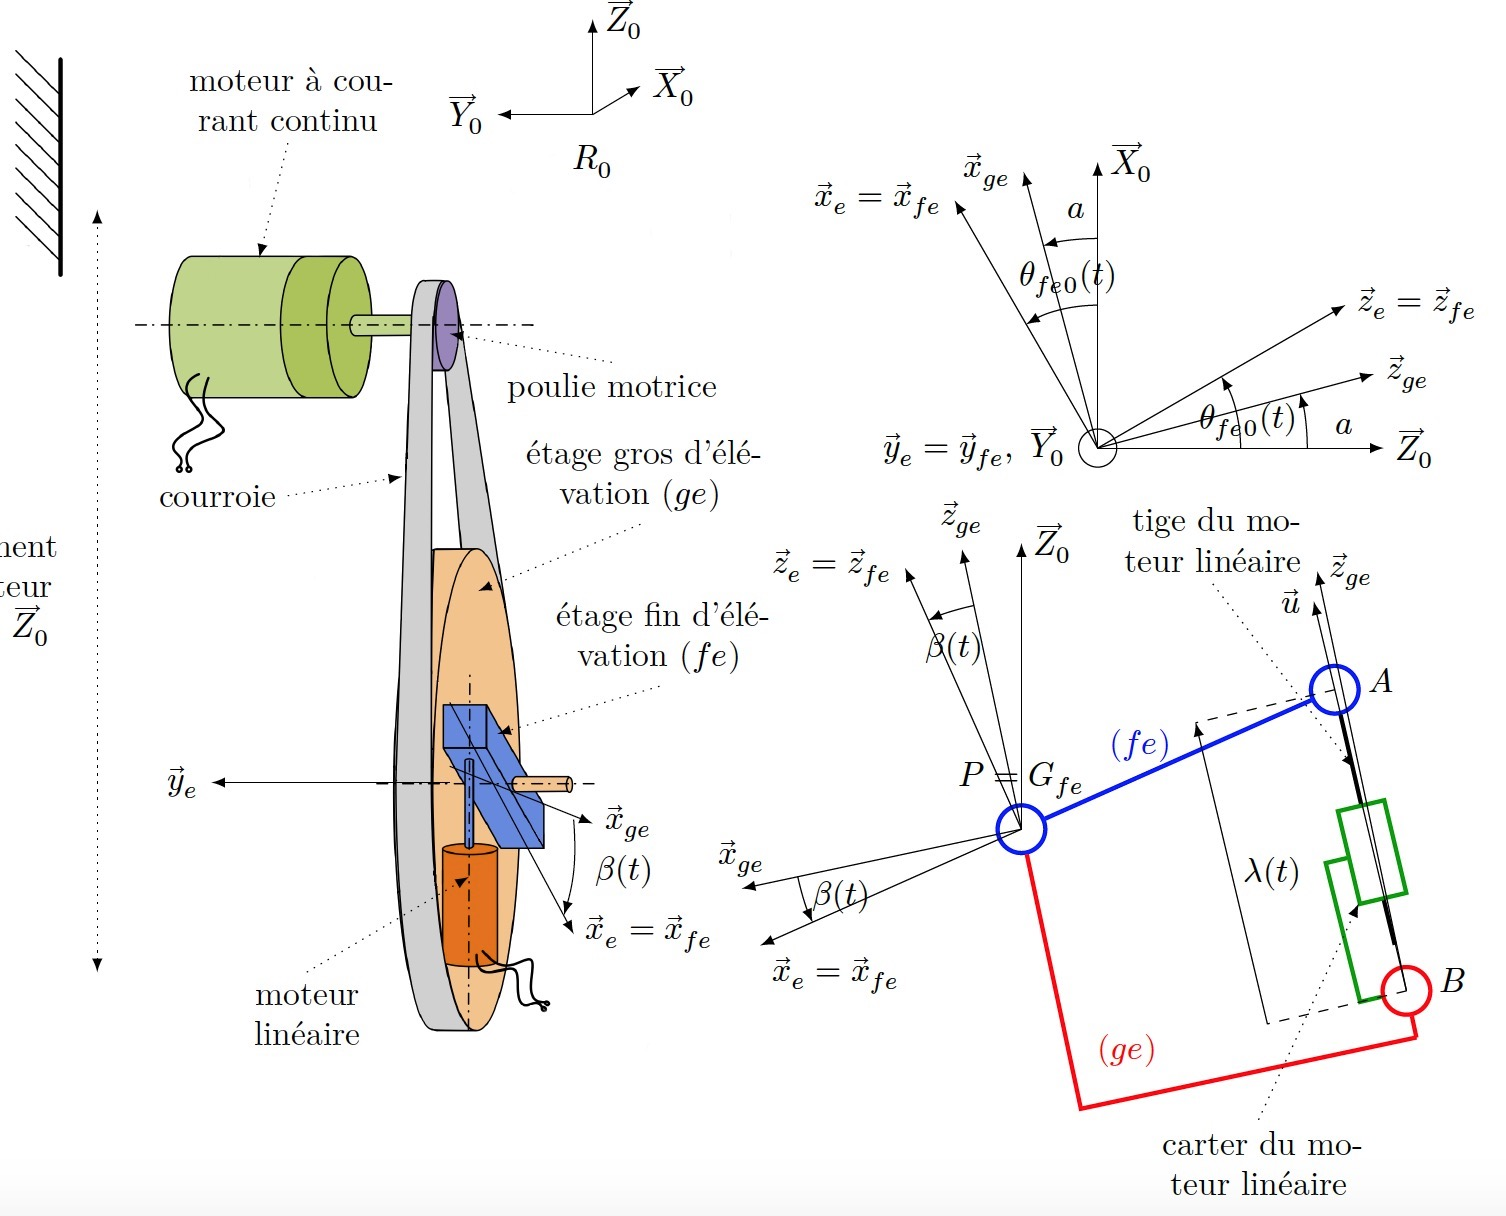
\includegraphics[width=0.9\textwidth]{figure14.jpg}
\caption{Structure et paramétrage des étages fin et gros de l'axe motorisé d'élévation \label{figure14}}
\end{center}
\end{figure}

\question{Exprimer le vecteur vitesse $\vect{V}(A\in fe/R_0)$ en fonction de $r$, $v(t)$ et $\dot{\theta}_{fe0}(t)$, puis en déduire une relation entre $v_{tige}(t)$ et $\dot{\theta}_{fe0}(t)$.}

Dans la suite du sujet, le passage dans le domaine symbolique de Laplace est noté de la façon suivante : $F(p)$
est la transformée de Laplace de la fonction $f(t)$, avec $p$ la variable de Laplace. Les conditions de Heaviside sont
vérifiées, c'est-à-dire que les valeurs initiales des fonctions temporelles sont nulles.

\question{En appliquant le théorème du moment dynamique à l'étage fin d'élévation ($fe$), exprimer littéralement la
fonction de transfert $\dfrac{\Omega_{fe0}(p)}{F_{mot}(p)}$ de la figure \ref{figure15} et en déduire les expressions de $M_{eq}$ et $K_1$. Effectuer les applications numériques.}

On rappelle que le gyromètre, placé directement sur l'étage fin d'élévation, permet de mesurer $\omega_{fe0\text{ mes}}(t)$. Son comportement peut être modélisé par un premier ordre de la forme $\dfrac{1}{1+\tau_{gyro}p}$ et de bande passante à $-3 dB$ égale à $100 Hz$.



\question{Calculer la valeur numérique de $\tau_{gyro}$.}

Le modèle d'asservissement de l'étage fin d'élévation étant établi, il est alors possible de concevoir sa commande.

%\FloatBarrier
\subsubsection{Conception de la commande de l'étage fin d'élévation}

Les performances de l'étage fin d'élévation ont été déterminées à partir des performances du FLIR établies en
partie \ref{partie1}. Elles sont données dans le tableau de la figure \ref{figure15}.

La consigne de vitesse $\dot{\theta}_{fe0\text{cons}}=\omega_{fe0\text{cons}}(t)$ est établie par rapport au référentiel galiléen $R_0$. Elle est calculée à partir de la détection de posture (DDP du casque TopOwl) de la tête du pilote et des informations
d'orientation du porteur par rapport au référentiel terrestre $R_0$ obtenues par la centrale inertielle du porteur.

\begin{figure}[!htb]
\begin{center}
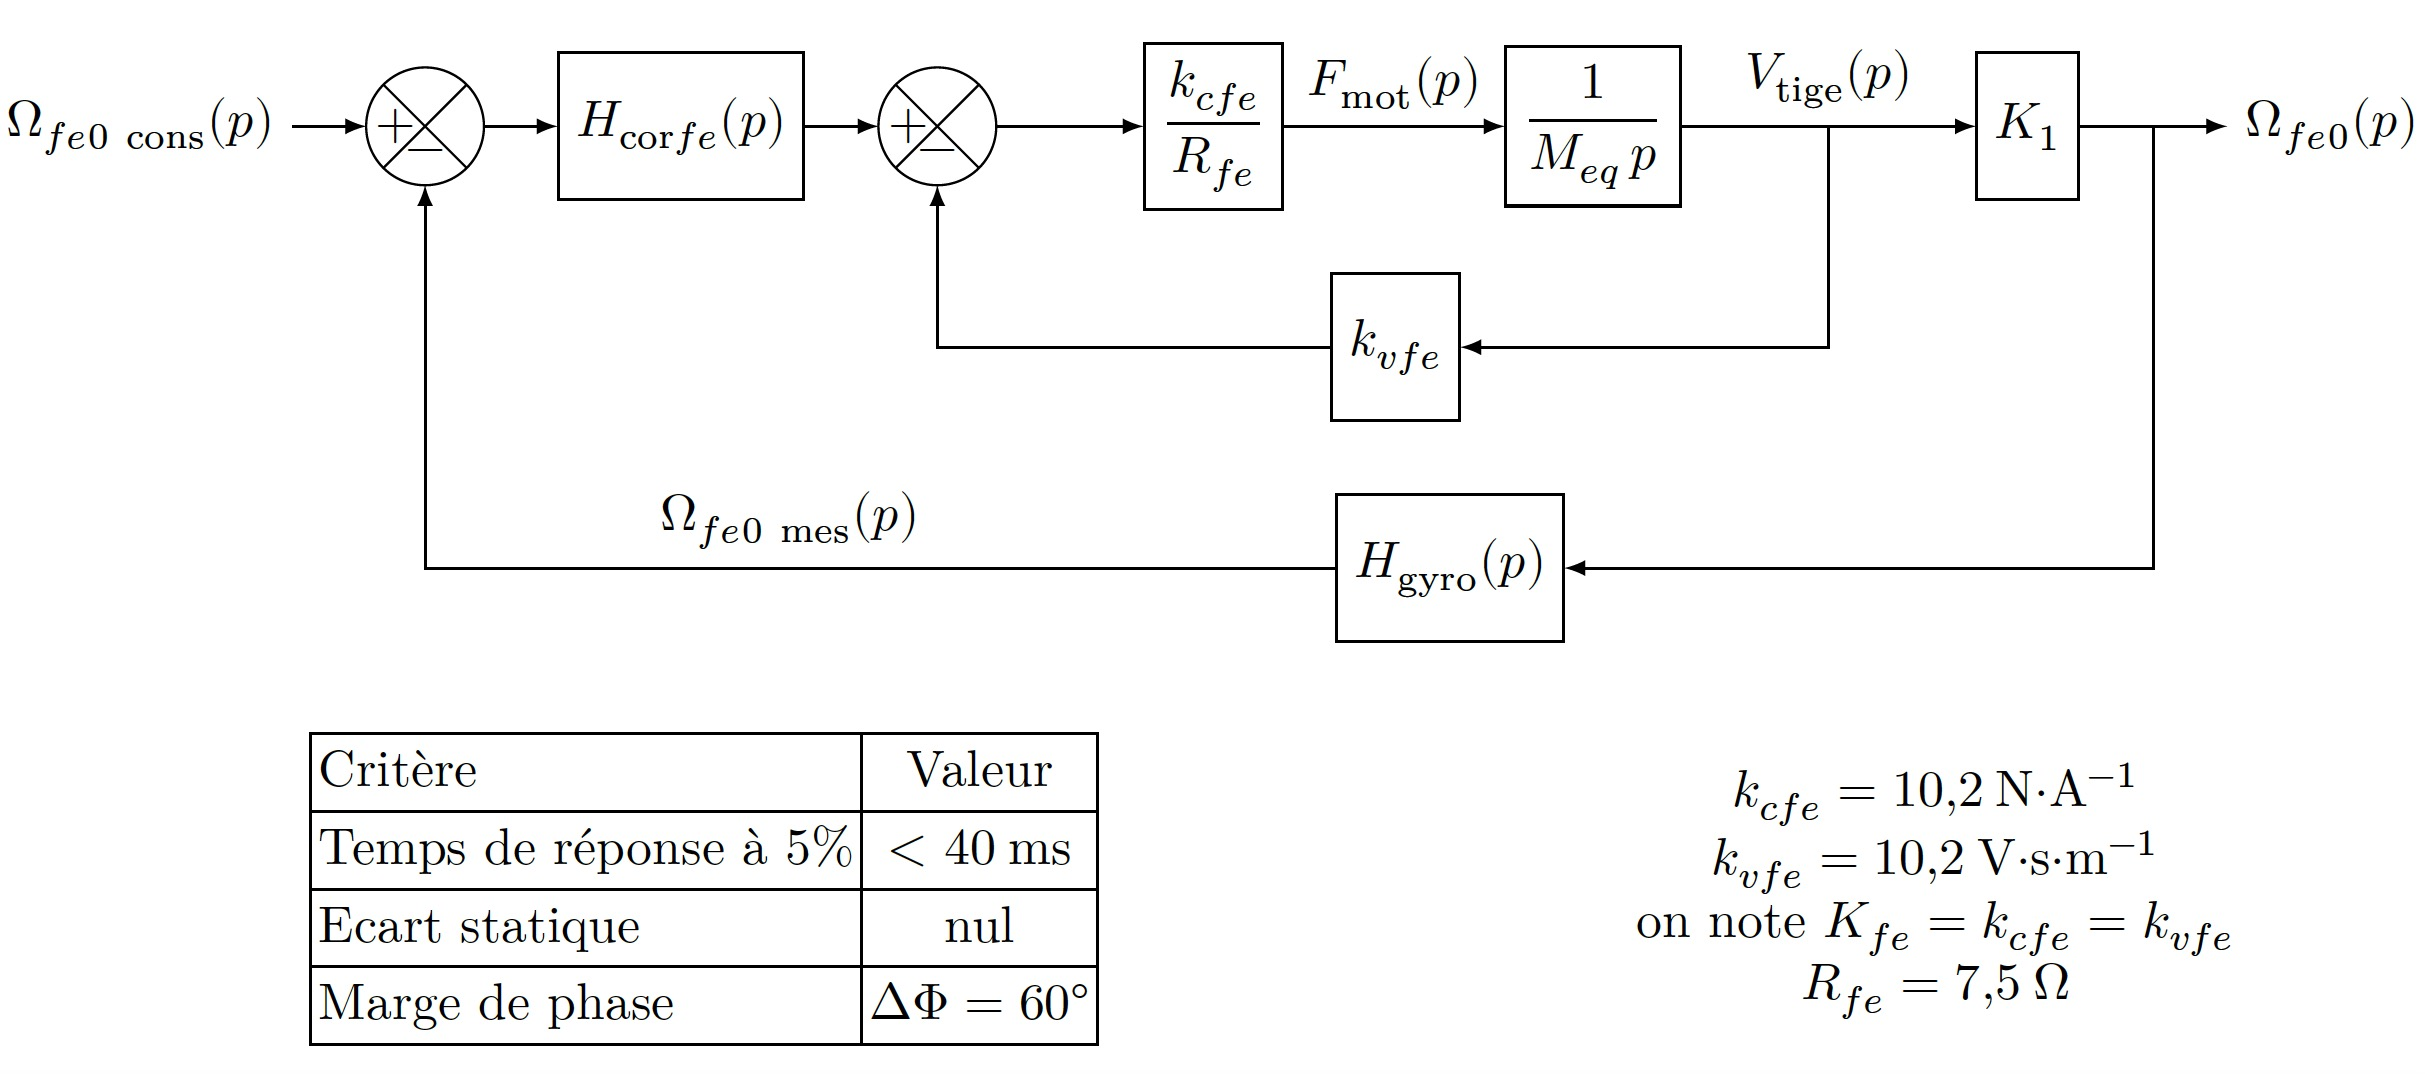
\includegraphics[width=0.9\textwidth]{figure15.jpg}
\caption{Modèle d'asservissement de l'étage fin d'élévation et performances attendues \label{figure15}}
\end{center}
\end{figure}

Dans un premier temps, l'asservissement de vitesse n'est pas corrigé, c'est-à-dire que $H_{corfe}(p)=1$.

\question{Exprimer littéralement et sous forme canonique la fonction de transfert $H_{fe1}(p)=\dfrac{\Omega_{fe0}(p)}{\Omega_{fe0cons}(p)}$, en fonction de $K_1$, $\tau_{gyro}$, $M_{eq}$, $K_{fe}$ et $R_{fe}$.}

Compte tenu des temps de réponse à observer, on montre que $H_{fe1}(p)$ peut se mettre sous la forme simplifiée
suivante :

\begin{align*}
H_{fe1}(p)\approx\dfrac{0,5}{1+3,65\times 10^{-1}p+6\times 10^{-4}p^2}
\end{align*}

\question{En utilisant l'abaque de la figure \ref{fig16}, déterminer le temps de réponse à $5\%$ et l'écart statique de
l'asservissement en vitesse de l'étage fin d'élévation en réponse à un échelon de vitesse unitaire. Conclure sur le
respect des performances en rapidité et en précision données sur la figure \ref{fig16}.}

\begin{figure}[!htb]
\begin{center}
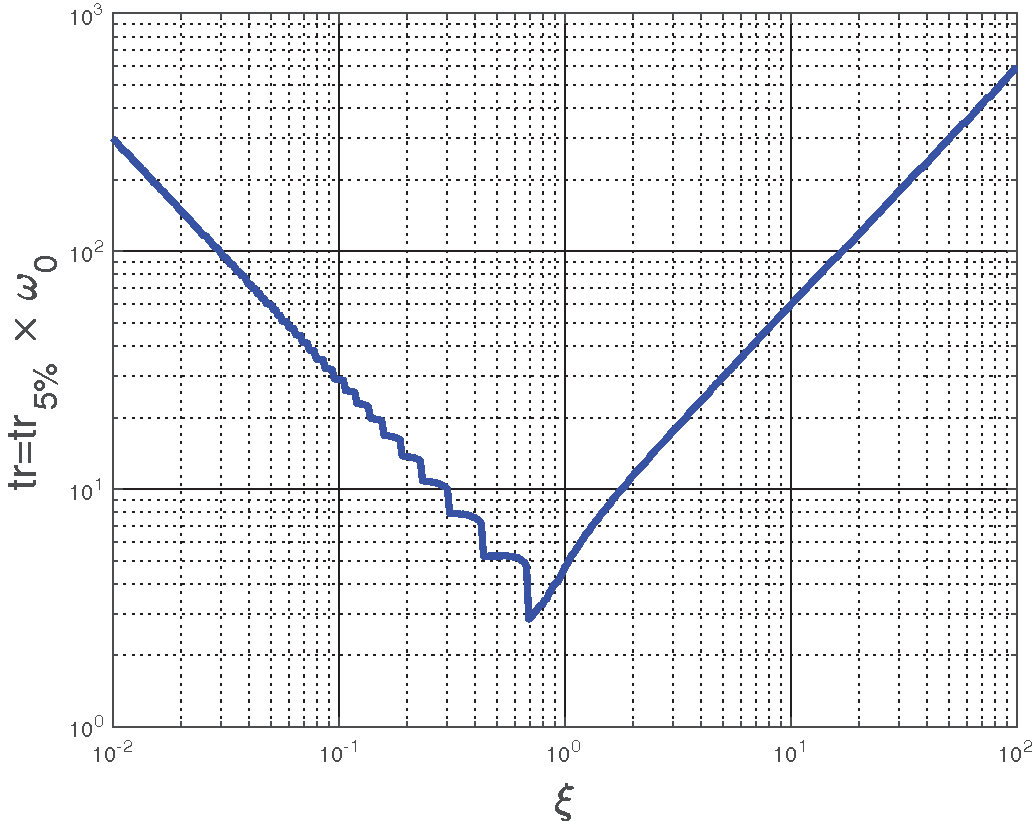
\includegraphics[width=0.6\textwidth]{amortissement.pdf}
\caption{Abaque des temps de réponse réduit\label{fig16}}
\end{center}
\end{figure}

On propose d'utiliser un correcteur proportionnel intégral de la forme $H_{corfe}(p) = K_{pfe}\left(1+\frac{1}{T_{ife}p}\right)$. La
fonction de transfert en boucle ouverte de l'asservissement en vitesse de l'étage fin d'élévation devient alors

\begin{align*}
H_{BOfe}(p)=K_{pfe}\left(1+\frac{1}{T_{ife}p}\right)\dfrac{1}{1+0,75p}\dfrac{1}{1+1,6\times 10^{-3}p}
\end{align*}

La figure \ref{figdr} du document réponse correspond aux tracés des diagrammes de Bode réels de $H_{BOfe}(j\omega)$ pour
$K_{pfe}=1$ et $T_{ife}= 0,1 s$, puis $T_{ife} = 0,01 s$.

\question{Sur cette même figure du document réponse, tracer le diagramme de phase asymptotique de $H_{BOfe}(j\omega)$
(Bode) pour $T_{ife}=0,1s$, en indiquant la pulsation $1/T_{ife}$.}



La lecture du tracé réel de la phase met en évidence un maximum à la pulsation $\omega_{max}$ telle que $\omega_{max}\in
\left[\dfrac{1}{T_{ife}}; 600\right] rad\cdot s^{-1}$.

\question{En supposant que le tracé réel semi-logarithmique de la phase est symétrique autour de $\omega_{max}$, calculer
la valeur de $T_{ife}$ comprise dans la décade $\left[0,01 s; 0,1 s\right]$ qui permet de régler ce maximum à $-120^{\circ}$.}


\question{Pour le réglage de $T_{ife}$ calculé à la question précédente avec $K_{pfe}=1$ et à partir des tracés réels du document réponse, calculer la valeur de $K_{pfe}$ qui permet de respecter le critère de marge de phase du tableau de la figure \ref{figure15}.}

Le modèle est complété en utilisant les réglages déterminés aux deux questions précédentes pour $K_{pfe}$ et $T_{ife}$. Afin de prendre en compte les caractéristiques du moteur linéaire, une saturation d'alimentation du moteur à 24 V est
ajoutée ainsi qu'une modification de la commande associée qui n'est pas étudiée ici et qui ne modifie pas les
réglages de $K_{pfe}$ et $T_{ife}$ déterminés précédemment. La réponse simulée $\omega_{fe0}(t)$ de l'étage fin d'élévation à une consigne de vitesse en échelon $\omega_{fe0cons}(t) = 1 rad\cdot s^{-1}$ est donnée sur la figure \ref{fig17}.

\begin{figure}[!htb]
\begin{center}
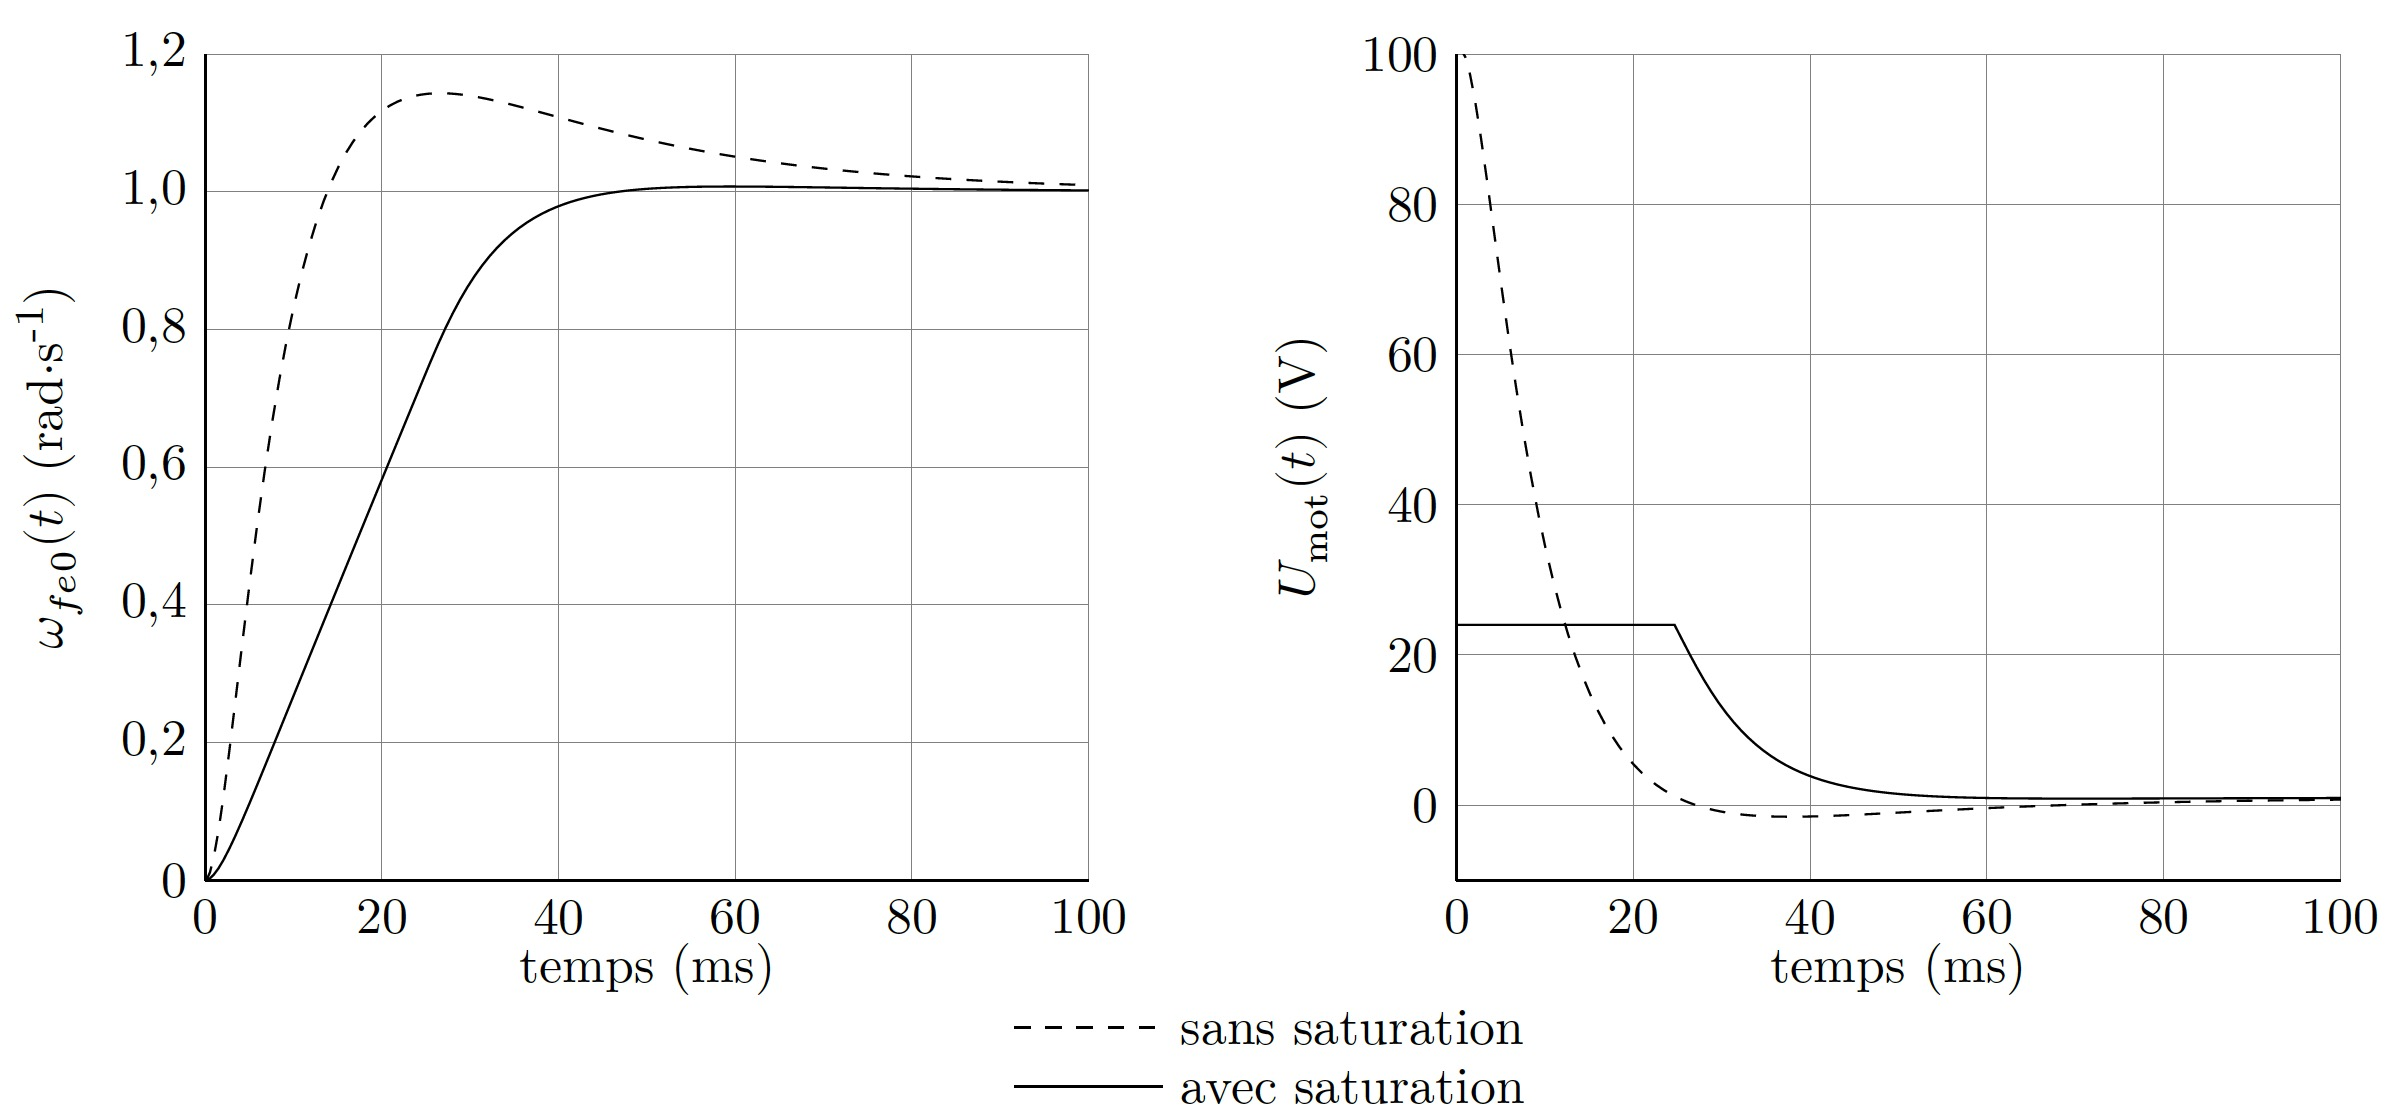
\includegraphics[width=1.0\textwidth]{figure17.jpg}
\caption{$\omega_{fe0}(t)$ et $U_{mot}(t)$ en fonction du temps avec et sans saturation de l'alimentation du moteur\label{fig17}}
\end{center}
\end{figure}

\question{D'après la figure \ref{fig17}, définir le temps pendant lequel la tension du moteur linéaire a été saturée et
expliquer les effets de cette saturation sur les performances simulées par rapport aux performances simulées
en gardant le modèle linéaire. Conclure sur la pertinence de la prise en compte de la saturation et sur les
performances de l'étage fin d'élévation.}

%\FloatBarrier
\subsubsection{Synthèse : validation des performances simulées du FLIR}

\begin{obj}
Simuler le comportement de l'axe motorisé d'élévation du FLIR et vérifier s'il respecte le cahier des
charges donné sur le tableau \ref{tab2}.
\end{obj}

À l'instar de l'étage fin d'élévation, l'étage gros d'élévation est également asservi, mais en position angulaire. Il
doit permettre à l'étage fin d'élévation de vérifier l'hypothèse émise précédemment, soit $\vect{u}\approx \vect{z}_e$, c'est-à-dire que l'angle $\beta(t)$ doit rester dans l'intervalle $\left[-5^{\circ}, +5^{\circ}\right]$.

Un capteur LVDT (Linear Variable Differential Transformer) permet de mesurer l'écart entre l'orientation de
l'étage fin d'élévation et l'étage gros d'élévation $\beta(t)=\theta_{fe0(t)}-\theta_{ge0}(t)$. Le modèle d'asservissement de l'axe
motorisé d'élévation est alors celui donné sur la figure \ref{fig18}.


\begin{figure}[!htb]
\begin{center}
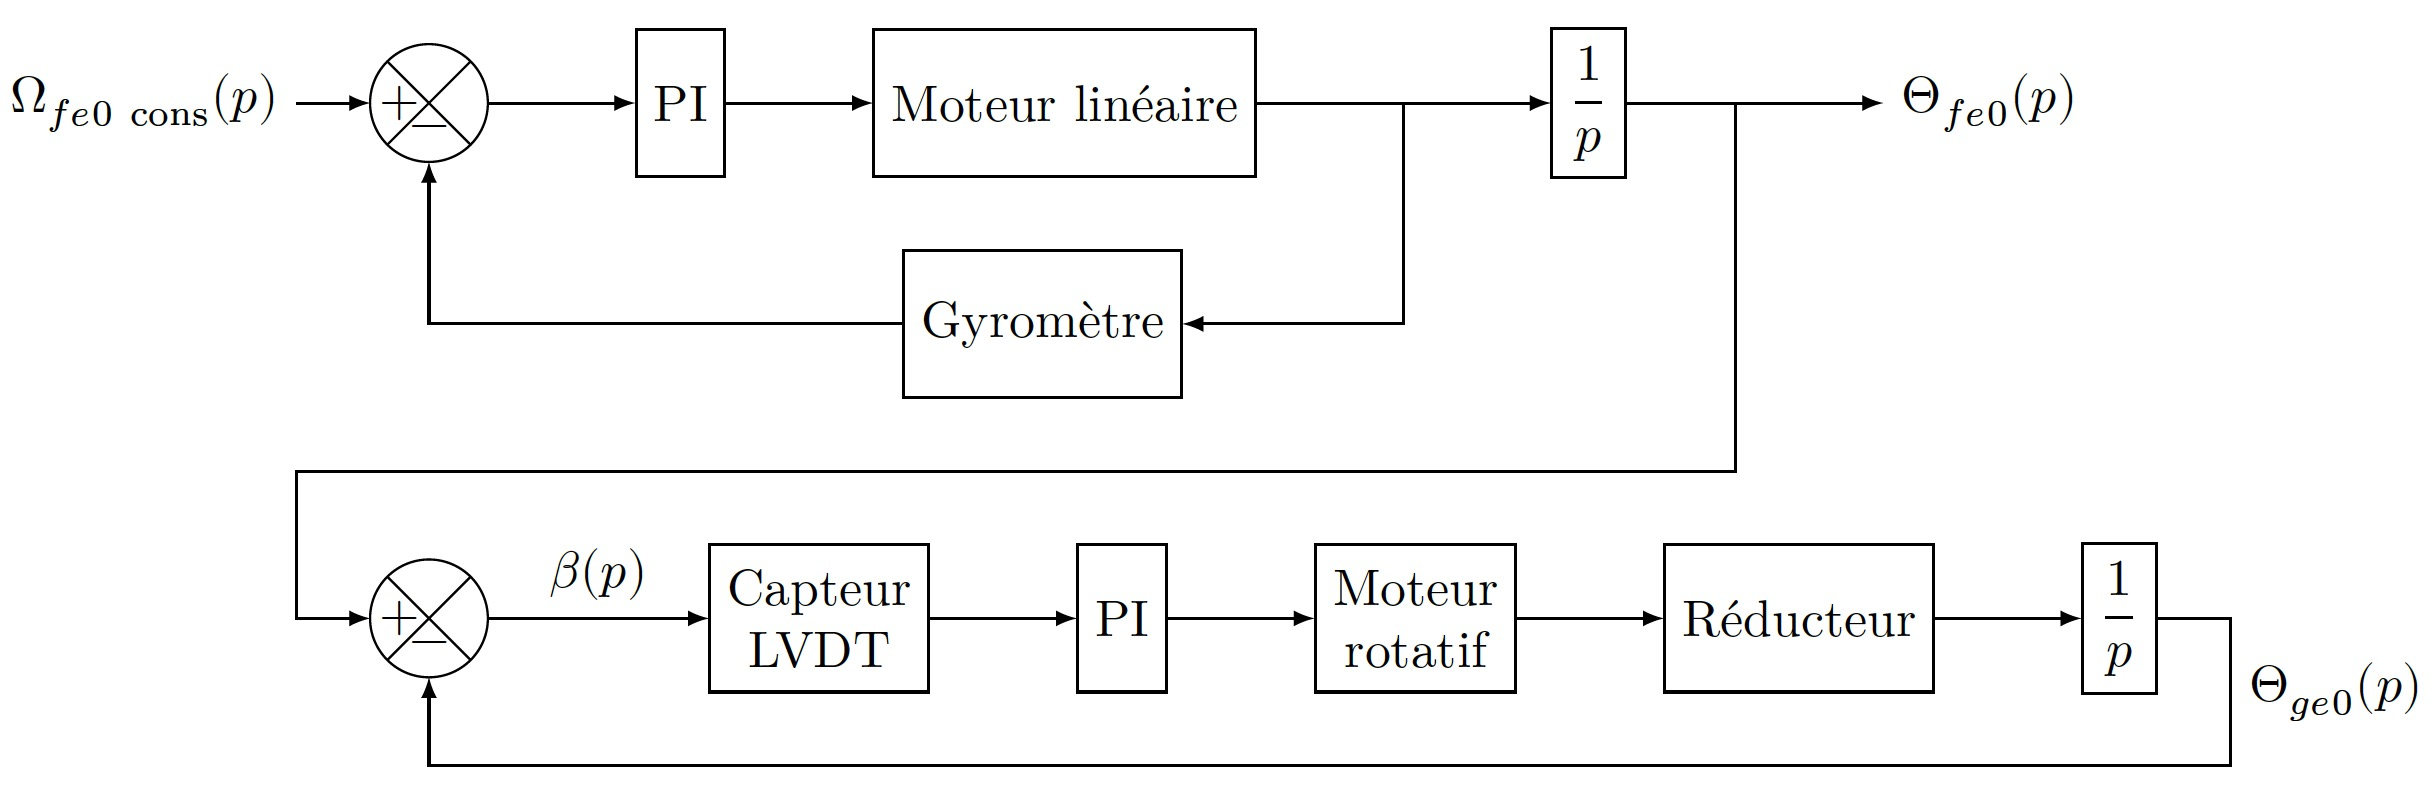
\includegraphics[width=1.0\textwidth]{figure18.jpg}
\caption{Modèle d'asservissement de l'axe motorisé d'élévation, PI représente un correcteur Proportionnel
Intégral \label{fig18}}
\end{center}
\end{figure}

La figure \ref{fig19} correspond à une mesure expérimentale du taux de rotation de la tête d'un pilote pour un mouvement
d'élévation de sa ligne de visée. Ce signal peut alors être utilisé comme signal de consigne envoyé à l'axe motorisé
d'élévation du FLIR.

\begin{figure}[!htb]
\begin{center}
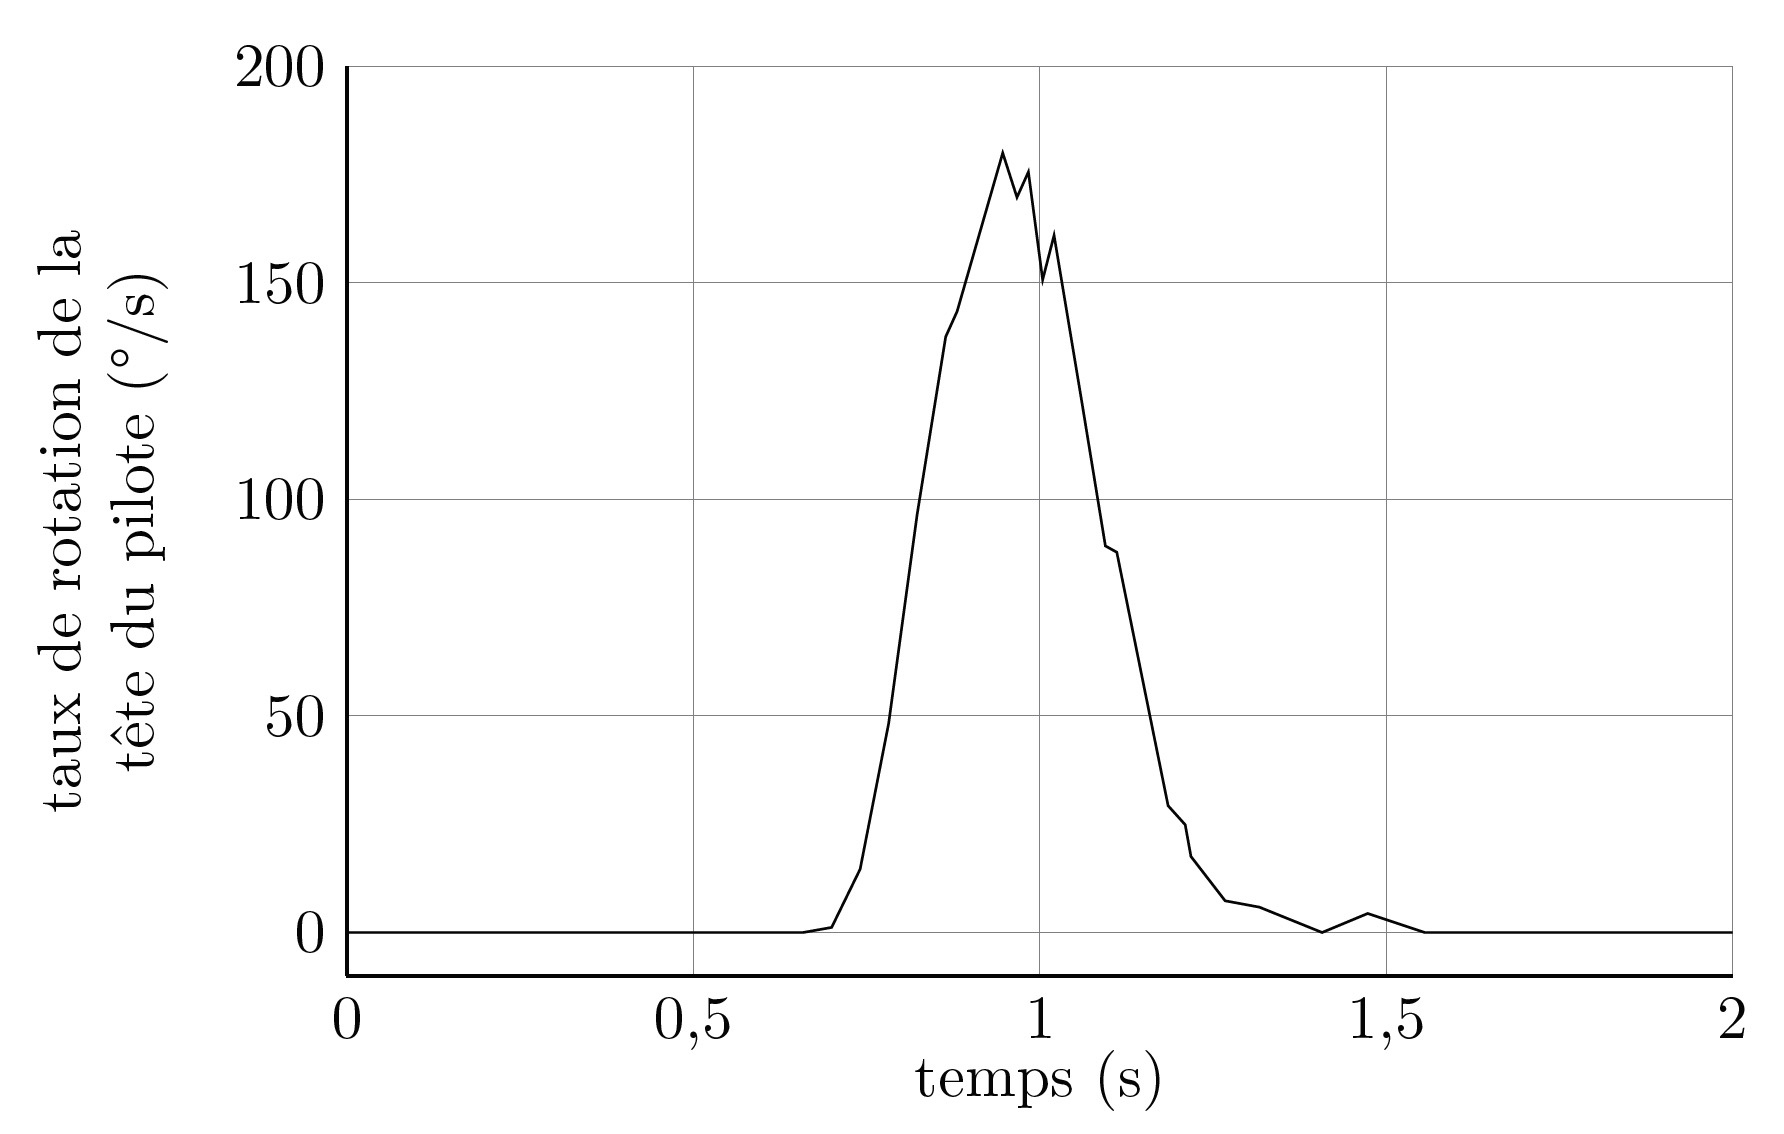
\includegraphics[width=1.0\textwidth]{figure19.jpg}
\caption{Mesure expérimentale du taux de rotation de la tête du
pilote (en degré par seconde) par rapport au référentiel galiléen, en
fonction du temps en seconde \label{fig19}}
\end{center}
\end{figure}

Pour simuler le modèle de l'axe motorisé d'élévation et comparer ses performances au cahier des charges du tableau \ref{tab2}, il est nécessaire de définir un signal de consigne $\omega_{fe0\text{ cons}}(t)$ composé des signaux canoniques utilisés
en automatique.

\question{À partir de la figure \ref{fig19} et en utilisant les signaux échelon et/ou rampe, proposer un modèle temporel
associé au signal de consigne $\omega_{fe0\text{ cons}}(t)$ exprimé en $rad\cdot s^{-1}$, sous la forme d'un tracé simple en fonction du temps en seconde. Tracer l'allure de $\theta_{fe0\text{ cons}}(t)$, exprimé en rad, qui correspond à l'évolution temporelle de la ligne de visée du pilote dans ce cas. Préciser les valeurs des points caractéristiques de ces deux courbes.}


\question{À partir des deux tracés précédents, indiquer quels critères du cahier des charges du tableau \ref{tab2} peuvent
être validés en utilisant ce signal de consigne dans la simulation du comportement de l'axe motorisé d'élévation
du FLIR. Après avoir dimensionné et implanté le correcteur proportionnel intégral (noté PI) au sein du modèle de l'étage
gros d'élévation (figure \ref{fig18}), on simule l'évolution de $\beta(t)=\theta_{fe0(t)}-\theta_{ge0}(t)$ pour le signal de consigne $\omega_{fe0\text{ cons}}(t)$ établi à partir de la mesure de la figure \ref{fig19}. Les résultats de simulation sont donnés sur la figure \ref{figB} du document réponse.}

\question{À partir de la figure \ref{figB} :}
\textit{
\begin{itemize}
\item vérifier si l'hypothèse $\vect{u}\approx \vect{z}_e$ reste valide ;
\item  pour chaque critère du cahier des charges du tableau \ref{tab2} et à l'aide de tracés sur le document réponse,
conclure sur l'aptitude du FLIR à respecter les performances du cahier des charges en comparant les valeurs
numériques mesurées sur les résultats de simulation à celles du tableau \ref{tab2}.
\end{itemize}
}